\chapter{Computação Ubíqua}
\label{ch:computacaoUbiqua}

\begin{quotation}[Mark Weiser, 1991]{Mark Weiser, 1991}
The most profound technologies are those that disappear.
\end{quotation}

A ideia de uma sociedade que pudesse conviver e, sobretudo, se comunicar com diversos dispositivos integrados e espalhados pelo ambiente com o objetivo de trazer grandes facilidades e comodidade ao homem não é tão recente. Tal cenário já foi mostrado em diversos filmes, relatado por escritores, filósofos e cineastas em suas obras futurísticas, onde os dispositivos eram capazes de entender o contexto das situações e, através de uma inteligência similar a humana, conseguir executar ações para interagir e colaborar com a sociedade.

Embora a ciência ainda esteja um pouco distante de atingir as perspectivas futurísticas dos filmes, existem diversos trabalhos sendo realizados para que um dia essa visão possa se tornar realidade. Este capítulo apresenta um breve histórico, introduz os principais conceitos da computação ubíqua,  as propriedades que a caracterizam, bem como discute contextos de uso para dispositivos móveis.      



\section{Histórico}
\label{sc:historico}

Motivados por antropólogos, filósofos e cientistas sociais, em meados de 1987, nos laboratórios do Xerox PARC, localizado no centro de pesquisa de Palo Alto, Mark Weiser e outros colaboradores deram início ao termo conhecido como Computação Ubíqua (\textit{Ubiquitous Computing}). Segundo \cite{campiolo2005} , a visão desses pesquisadores se distanciava do esquema tradicional: uma pessoa, um computador pessoal. O propósito da equipe era exatamente espalhar dispositivos com capacidades computacionais pelo ambiente, entretanto, sem que a presença destes fosse percebida, daí então o termo Computação Invisível. 

Posteriormente, em 1991, Mark Weiser formalizou seu estudo publicando  seu primeiro artigo referente ao assunto na Scientific American, a este ele deu o título \textit{The Computer for the 21th Century} \citep{weiser1991}. Neste artigo, além de  apresentar a comunidade acadêmica uma nova linha de pesquisa até então inexplorada, foi mostrada como deveria ser implementada, bem como quais seriam as expectativas com relação à computação ubíqua. Em 1993, Weiser também publicou o artigo \textit{Some Computer Science Issues in Ubiquitous Computing} \citep{weiser1993}, trazendo outras questões relevantes de computação ubíqua, bem como abordando outras questões referentes a hardware, rede, privacidade, aplicações, interações e métodos computacionais. 

De acordo com \cite{campiolo2005}, mesmo com estas publicações e outras pesquisas relacionadas, o assunto não teve destaque durante a década de 90. Impulsionados pela internet, nessa década, o enfoque das pesquisas foram os sistemas distribuídos. Todavia, este fato fez com que a computação ubíqua também tivesse um avanço, haja vista que muitas das limitações, principalmente se tratando de questões relacionadas a comunicação, foram resolvidas devido a pesquisas em sistemas distribuídos e sistemas de telecomunicações. Segundo \cite{campiolo2005}, somente a partir do final da década de 90, impulsionado pela evolução dos dispositivos eletrônicos, ainda menores e com capacidades computacionais cada vez maiores, bem como pela computação móvel, o assunto veio à tona novamente.  Ainda segundo \cite{campiolo2005}, um outro passo importante para a evolução da computação ubíqua foi o advento de eventos científicos específicos, por exemplo, o \textit{Ubicomp – ACM} (referencia), e o surgimento de revistas também específicas, tendo destaque a  \textit{IEEE Pervasive Computing} (referencia).  

Nesse ínterim, conceitos foram introduzidas, outros campos relacionados foram descobertos, bem como a área foi ganhando força com o surgimento de diversos grupos de pesquisas. Alguns desses conceitos são apresentadas na próxima subseção. 


\section{\textit{Ubiquitous Computing}}
\label{sc:definicoes}

Esta seção tem o proposito de expor uma visão geral da Computação Ubíqua (do inglês \textit{Ubiquitous Computing - UC}), apresentado alguns de seus conceitos, bem como descrevendo os principais requisitos das aplicações com esse paradigma.

De acordo com a visão de \cite{weiser1991,weiser1993},  computação ubíqua é um paradigma no qual a computação é profundamente integrada, onde os ambientes são impregnados de dispositivos, tendo estes capacidade de computação e comunicação, os quais devem ser inseridos de modo transparente, isto é, de maneira invisível, às atividades cotidianas dos usuários. Nesses trabalhos,  Weiser afirma que as tecnologias que possuem maior destaque são aquelas que desaparecem ao se tornar parte do cotidiano do usuário, impossibilitando, portanto, perceber sua presença.

Segundo \cite{poslad2009}, a computação ubíqua representa uma poderosa mudança na computação, onde as pessoas vivem, trabalham e se divertem em ambientes cheios de dispositivos intercalados ao mundo. Poslad afirma, também, que a computação ubíqua postula um mundo onde as pessoas são cercadas por dispositivos e uma infraestrutura computacional que nos apoia em tudo que fazemos. 

\begin{figure}[htp]
\begin{center}
  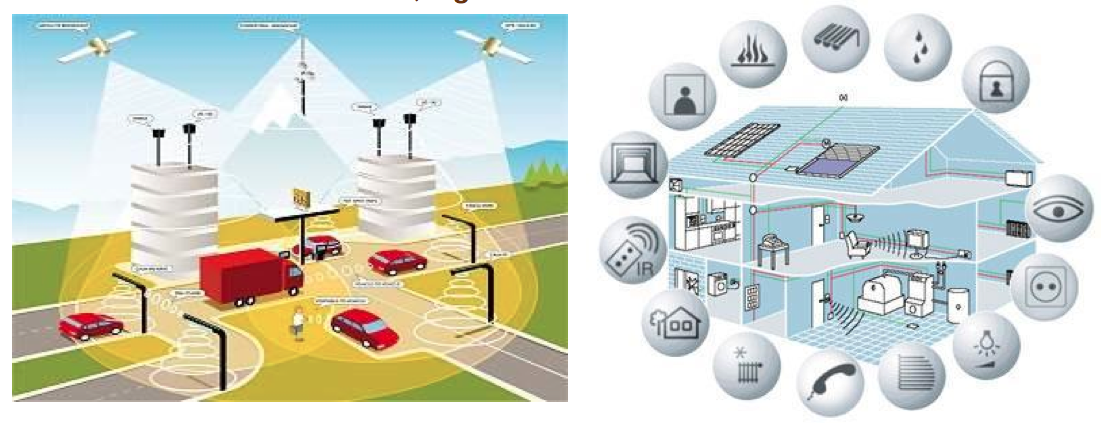
\includegraphics[width=14cm]{images/cenario_ubiquo.png}
  \caption[Ilustração de um cenário ubíquo]{Ilustração de um cenário ubíquo.}
  \label{fig:exampleFigCenarioUbiquo}
\end{center}
\end{figure}

Ainda de acordo com \cite{poslad2009}, existem três requisitos fundamentais na Computação Ubíqua que fora idealizada por Mark Weiser: computadores precisam estar distribuídos, interligados e acessíveis de forma transparente; a interação humano-computador deve ser escondida ou, simplesmente, minimizada; para que os sistemas possam otimizar suas operações nos diversos ambientes dinâmicos em que operam, esses precisam ser sensível ao contexto.  O autor ainda considera outros dois requisitos adicionais como sendo, também, fundamentais: computadores devem operar de maneira automática; computadores devem lidar com  múltiplas ações dinâmicas. 
	
Segundo \cite{lopes2011}, uma das principais características dos sistemas ubíquos são os ambientes altamente dinâmicos  nos quais estes estão inseridos. Para Lopes, nesses ambientes dinâmicos, diversos dispositivos, de natureza diferente ou não, interagem entre si com a finalidade de fornecer informações relevantes que, de algum modo, possa contribuir com as atividades cotidianas dos usuários de maneira imperceptível.
	
Isto posto, a computação ubíqua é a computação onipresente, isto é, acessível em todos os lugares, conforme apresentado na figura \figref{fig:exampleFigCenarioUbiquo}, que tem o propósito de facilitar a interação entre usuários e dispositivos computacionais espalhados pelo ambiente, de modo que esses usuários não percebam que estão fornecendo comandos para os computadores que os cercam.  Em outras palavras, é a computação por meio da comunicação entre usuários, dispositivos e ambientes, objetivando simplificar e, sobretudo, facilitar a realização das tarefas cotidianas dos usuários sem que estes percebam.


\section{Propriedades}
\label{sc:propriedades}
Hodiernamente, na literatura, podemos encontrar um grande número de requisitos da computação ubíqua. Todavia, para efetivamente caracterizar o ideal que fora criado por Weiser, pesquisadores espalhados por todo mundo documentam, em suas publicações acadêmicas, as propriedades essenciais para o verdadeiro cenário ubíquo \citep{gomes2007}. 

Esta seção tem o propósito de apresentar uma coleção dos requisitos mais relevantes da computação ubíqua. 

\subsection{Sensibilidade ao Contexto}
Uma das principais áreas de pesquisa dentro da computação ubíqua é a computação sensível ao contexto  \citep{carmo2012}. Segundo \cite{schilit1994}, o primeiro a apresentar uma definição para o termo, a computação sensível ao contexto é “\textit{o estudo de aplicações que se adaptam de acordo com a localização do usuário, grupo de pessoas, objetos próximos ao usuário e as mudanças ocorridas com esses objetos ao longo do tempo}”. A partir desse ponto, surgiram diversos conceitos, de diversos autores, mas sempre conceituando o termo de forma bastante semelhante:

\begin{itemize}
\item Aplicações que conseguem modificar ou adaptar seu comportamento dinamicamente baseado nas informações de contexto do usuário ou da aplicação \citep{ryan1997}.
\item Sistema que se utiliza de informações relativas ao contexto para fornecer, de alguma maneira, serviços ou informações relevantes ao usuário \citep{dey2000}.
\item Aplicações que se beneficiam da descoberta de informações de contexto tais como: localização do usuário, hora do dia, dia da semana, temperatura, dispositivos próximo ao usuário, etc. objetivando melhorar o desempenho de aplicações computacionais \citep{chen2000}.
\end{itemize}

Sabemos que Sistemas de Computação Ubíqua são integrados com o ambiente. Nesse sentido, esses sistemas precisam utilizar informações de contexto para proporcionar adaptações no comportamento e, sobretudo, nas funcionalidades do próprio sistema \citep{tandler2004}. Dessarte, essa característica permite não só que o sistema conheça o ambiente no qual está operando, mas que ele possa, também, se ajustar automaticamente de acordo com o contexto sem ao menos necessitar que o usuário esteja ciente desse ajuste.            

\subsection{Invisibilidade}
Muitos definem computação ubíqua também como computação invisível \citep{gomes2007}, e isso não é por acaso. Segundo \cite{weiser1991}, quanto mais uma tecnologia está presente em nossas vidas, menos perceptível ela se torna.  Nesta visão, o computador passa a se tornar fundamental na realização das principais atividades do dia-a-dia do usuário, todavia, dilui-se no mundo físico de tal forma que passa a se tornar, também, tão presente e imperceptível quanto o ar que se respira \citep{gomes2007}.

De acordo com \cite{queirozfilho2012}, esta propriedade pode ser interpretada em dois sentidos: o primeiro refere-se a miniaturização dos dispositivos computacionais, bem como a capacidade destes em se incorporar aos objetos do dia-a-dia (e.g. móveis, vestimentas, equipamentos médicos, etc.), tornando-se,  assim, fisicamente invisível para as pessoas;  a segunda interpretação refere-se a forma como os dispositivos conseguem trabalhar sem desviar a atenção do usuário e, por conseguinte,  tornando-os imperceptíveis.  Nesse sentido, apesar da tecnologia estar visível fisicamente ela consegue realizar duas funções sem necessitar da atenção dos usuários.  

\subsection{Interoperabilidade espontânea}
Em \cite{kindBerg2012}, os autores apontam a interoperabilidade espontânea como um das características fundamentais dos sistemas ubíquos. Além disso, eles afirmam que um sistema ubíquo é composto por componentes de infraestrutura e dispositivos computacionais heterogêneos que usam tecnologias diferentes, bem como oferecem funcionalidades diferentes e, portanto, a interoperabilidade espontânea é vista como uma característica desejável a implementação da computação ubíqua exatamente pelo fato da possibilidade de integração dinâmica entre esses componentes e dispositivos. 

Isto posto, a partir desta propriedade, dispositivos e serviços podem interagir de maneira automática e, sobretudo, sem intervenção do usuário, compartilhando recursos ou, simplesmente, trocando informações, permitindo, deste modo, uma completa integração entre os dispositivos espalhados pelo ambiente. 

Seja um ambiente ubíquo implementado em uma estação de ônibus de uma determinada cidade. A interoperabilidade espontânea pode ser observada se, por exemplo, o ônibus é capaz de transferir  para os usuários informações sobre horários, pontos e acontecimentos no seu percurso sem qualquer intervenção manual para configurar o dispositivo do usuário. Ou seja, a interoperabilidade espontânea  é caracterizada pela capacidade de um sistema se comunicar de forma transparente com outro sistema sem a necessidade de intervenção do usuário.


\subsection{Integração Física}
A integração física, assim como a interoperabilidade espontânea, é considerada uma das características fundamentais dos sistemas ubíquos \citep{kindBerg2012}. De acordo com \cite{gomes2007}, os espaços inteligentes, do inglês \textit{smart spaces}, se caracterizam pela intensa colaboração entre elementos computacionais e componentes do mundo físico. 
	
Com o objetivo de exemplificar tal integração, os autores de \cite{kindBerg2012} citam o projeto denominado MediaCups \citep{mediacups2001}, onde uma xícara de café inteligente, além de servir como uma xícara de maneira usual, contém elementos como sensores, recursos de processamento e rede, que acabam permitindo que ela possa comunicar seu estado (e.g. cheio, vazio, frio, morno, etc.) ao seu proprietário. 
	
Nesse sentido, a integração física é justamente a ideia de que elementos computacionais se unam a componentes físicos rotineiramente utilizados pelas pessoas para que, através dessa colaboração, este conjunto possa trazer benefícios e, sobretudo, melhorar a interação com seu usuário.

\subsection{Adaptação e Tolerância a falhas}
Levando em consideração a grande dinamicidade existente na Computação Ubíqua, conforme já mencionado na seção \ref{sc:definicoes}, os sistemas ubíquos precisam adaptar suas configurações em tempo de execução para acompanhar ativamente as mudanças ocorridas no ambiente \citep{lopes2011}. Todavia, os sistemas precisam levar em consideração não somente as mudanças de contexto, mas, sobretudo, as falhas que podem ocorrer nos serviços disponíveis, na rede ou até mesmo nos dispositivos, bem como ter a capacidade de se adaptar, também, à essas falhas para que a parada ou travamento do sistema possa ser evitada.

Nesse sentido, essa capacidade de tolerar possíveis falhas fornece aos sistemas a possibilidade de manter o seu funcionamento exatamente como fora especificado mesmo mediante a ocorrência de falhas.     

\subsection{Interfaces naturais}
De acordo com \cite{gomes2007}, em \textit{smart-spaces}, faz-se necessário a busca por técnicas que permita a utilização de recursos comumente utilizados no dia-a-dia das pessoas, tais como  gestos, voz e até mesmo olhares como meio de comunicação entre homem e  máquina. Isto é, a ideia é exatamente levar elementos digitais ao mundo real, mas de maneira tão sutil que acaba não influenciando tanto na maneira como determinada atividade é realizada pelo usuário e, sobretudo, fazendo com que tal interação seja simples e natural.

\section{Contextos de Uso}
\label{sc:contextoDeUso}
Uma importante área de pesquisa dentro do domínio de dispositivos móveis é o que vem sendo denominado de contexto de uso \citep{carmo2012}. Este conceito tem como propósito trazer melhorias à experiência do usuário na utilização de dispositivos móveis.  

A ideia é coletar informações durante o uso do dispositivo, de maneira imperceptível para o usuário, que permita reconhecer o cenário atual.  Assim, ao identificar o contexto, é possível fornecer serviços que sejam de interesse para o usuário no momento e no cenário de uso e, por conseguinte, melhorar  sua experiência ao utilizar o dispositivo.

Em outras palavras, o objetivo é fazer com que um determinado dispositivo possa se adaptar às diversas situações de uso de modo a atender a necessidade do usuário no momento. Para exemplificar, suponhamos que um determinado usuário tenha o costume de correr todos os dias no parque ou na praia, e que quando ele está no parque gosta de ouvir um tipo de música diferente de quando ele está correndo na praia. Ao coletar informações de contexto referentes a atual localização do usuário,  o dispositivo poderia adaptar de forma automática sua interface, de modo que as músicas que o usuário costumeiramente escuta no local possa tocar no dispositivo. 


\chapter{\textit{Crowdsourcing}}
\label{ch:crowdsourcing}

\begin{quotation}[Daren C. Brabham, 2008]{Daren Brabham, 2008}
Crowdsourcing is a model for problem solving, not merely a model for doing business.
\end{quotation}

Este capítulo apresenta uma técnica para solucionar problemas através do conhecimento coletivo denominada \textit{Crowdsourcing}, mostrando seus principais conceitos e definições, bem como discutindo os três principais desafios dessa técnica: o recrutamento, o projeto de tarefas e o controle de qualidade. Por fim, a Gamificação é mostrada como uma das soluções para os principais problemas enfrentados no uso de  \textit{Crowdsourcing}.

\section{\textit{Crowdsourcing}}
\label{sc:crowdsourcing}

De acordo com \cite{brabham2008}, \textit{Crowdsourcing} é um modelo de produção para solucionar problemas com base na inteligência e, sobretudo, conhecimento coletivo. Segundo \cite{schenk2009}, o termo é um neologismo derivado das palavras Crowd (multidão) e Outsourcing (terceirização) e tem o objetivo de subcontratar um grande número de indivíduos anônimos a fim de resolver desafios.  Conforme \cite{Paraschakis2013}, o termo \textit{crowdsourcing} foi popularizado por Jeff Howe em seu artigo “\textit{The rise of crowdsourcing}” \citep{howe2006} da revista Wired, onde o jornalista mostrou a situação vivida por muitas empresas que buscavam aproveitar a participação coletiva para seu próprio empreendimento.  

Segundo \cite{Hu2012}, \textit{crowdsourcing} é um convite aberto para recrutar uma multidão de pessoas para resolver um problema em conjunto. Em termos gerais, isto pode ser considerado um meio de agregação de trabalho a partir de uma quantidade massiva de pessoas \citep{surowiecki2005}. Ademais, para \cite{pintado2011},  esse modo de produção colaborativa realizada por esse grande número de usuários não possui nenhuma forma de gestão formal.

Em \cite{pintado2011}, a Wikipedia é mostrada como exemplo do uso de inteligência coletiva e \textit{crowdsourcing}. Inicialmente chamada de Nupedia, o objetivo de seus fundadores era criar uma enciclopédia virtual através da colaboração de profissionais das mais diversas áreas. Contudo, a burocracia existente na aprovação de cada verbete sinalizou que o projeto não seria viável desse modo. Então, foi criado um novo site e, desta vez, permitindo que qualquer pessoal, seja esta profissional ou não, pudesse criar, bem como alterar o conteúdo dos verbetes. O resultado foi a criação de milhares de verbetes em poucos meses após a mudança. A ação de editar ou criar um verbete era tão simples, rápida e intuitiva que as pessoas se sentiam motivadas a participarem do projeto \citep{pintado2011}. Assim, o esforço coletivo desempenhado por milhões de colaboradores propiciou a criação da maior enciclopédia virtual, onde os verbetes seguem sendo atualizados até hoje.   

Para \cite{pintado2011}, o \textit{crowdsourcing} se configura, portanto, “\textit{como uma rede global de talentos que não necessariamente leva em consideração as vias formais de especialização}”, o que de acordo com \cite{surowiecki2005} e [Howe 2009], não causa perda de qualidade da informação gerada. Pelo contrário, conforme  \cite{surowiecki2005}, fatores relativos à coletividade são determinates para o sucesso desse processo. As propriedades das soluções de \textit{crowdsourcing} eficazes são descritas por ele no livro \textit{The Wisdom of Crowds} \citep{surowiecki2005}: 

\begin{enumerate}
\item \textbf{Diversidade de opinião}: "cada pessoa deve ter alguma informação pessoal, mesmo que seja apenas uma interpretação excêntrica dos fatos conhecidos." 
\item \textbf{Independência}: "As opiniões das pessoas não são determinadas pelas opiniões dos que os rodeiam." 
\item \textbf{Descentralização}: "as pessoas são capazes de se especializar e trabalhar com conhecimento local. "
\item \textbf{Agregação}: "a existência de algum mecanismo para transformar avaliações pessoais em decisões coletivas."
\end{enumerate}

Ainda segundo \cite{surowiecki2005}, uma multidão heterogênea pode sugerir uma grande quantidade de soluções diferentes para um determinado problema, o que pode ser extremamente difícil para um grupo de profissionais onde as expertises são mais homogêneas. No entanto, para que os sistemas de \textit{crowdsourcing} sejam eficazes, é necessário estar atento a três problemas críticos \citep{Hu2012}:  disponibilidade da multidão (recrutamento), projeto de tarefas e controle de qualidade. Em primeiro lugar, os sistemas de \textit{crowdsourcing} precisam recrutar pessoas para executar as tarefas; em segundo lugar, as tarefas devem atender a especialização, tempo disponível e, sobretudo, esforço dos colaboradores; por fim, os sistemas precisam assegurar que os usuários completaram as tarefas de maneira correta. Por exemplo, a natureza das tarefas, normalmente, está diretamente relacionada ao tamanho, a motivação e ao possível viés da população potencial \citep{Hu2012}. Estes três problemas são discutidos separadamente nas seções subsequentes.

\subsection{Recrutamento}
Para \cite{Hu2012}, quaisquer sistema de \textit{crowdsourcing} deve, primeiramente, recrutar pessoas para desempenhar suas tarefas. Todavia, encontrar essas pessoas nem sempre é algo tão simples. O recrutamento geralmente fica mais difícil quando as tarefas são mais complexas. Por exemplo, encontrar pessoas que possam descrever os objetos existente em uma determinada foto é algo relativamente fácil \citep{Von2004}, enquanto que encontrar pessoas que possam traduzir um documento de uma determinada língua para outra \citep{Zaidan2011} pode não ser uma missão tão simples. Nesse sentido, conforme \cite{Hu2012}, é mais fácil encontrar colaboradores se as tarefas de um sistema envolvem apenas as habilidades diárias. Isto é, se todo mundo tem as habilidades para realizar as tarefas, tais sistemas possuem uma população muito grande para recrutar. 

Enquanto a tarefa de compreender e descrever as imagens é um problema muito difícil de se resolver computacionalmente  \citep{Von2004}, é uma tarefa bastante fácil para a maioria dos seres humanos. Assim, o sistema criado por  \cite{Von2004}, cujo principal objetivo é compreender e descrever imagens conseguiu atrair uma grande quantidade de colaboradores. Não obstante, recrutar usuários com habilidades menos comuns é mais difícil, haja vista que nem todo mundo é capaz de realizar determinadas tarefas. Por exemplo, no trabalho realizado por \cite{Zaidan2011} , onde o objetivo era fazer com que vários documentos fossem traduzidos de uma língua para outra através do trabalho coletivo, o usuário precisa saber  falar, no mínimo, duas línguas diferentes.

Para determinadas tarefas o recrutamento se torna ainda mais difícil, pois é necessário que o usuário, além de disponível, esteja motivado à colaborar. Por exemplo,  para fazer com que usuários possam notificar possíveis incidentes ocorridos no trânsitos (e.g. engarrafamentos, acidentes, barreiras e etc.) a fim de alertar a população, além do usuário precisar estar vivenciando ou, ao menos, ciente do incidente, é preciso fazer com que este sinta-se motivado a colaborar com a divulgação dessa informação.  Isto é, para algumas tarefas a disponibilidade da multidão é um grande problema, pois é mais difícil encontrar pessoas dispostas e motivadas \citep{Hu2012}. 

Uma solução comum é o emprego de pagamento de bônus para os bons colaboradores, de modo a mantê-los presentes e ativos no sistemas, bem como atrair e motivar novos usuários \citep{Hu2012}. Uma técnica muito utilizada para o engajamento de usuários em diversos sistemas de \textit{crowdsourcing} é conhecida como Gamificação, e é apresentada na próxima seção.   


\subsection{Projeto de Tarefas}
O projeto  de tarefas no crowdsoursing é considerado uma questão central, pois, assim como o recrutamento, está intimamente ligada à motivação do usuário, bem como a qualidade dos resultados \citep{Hu2012}. 

Segundo \cite{Hu2012}, muitas tarefas são projetadas de modo a fazer com que o usuário perceba que está colaborando, bem como pode estar diretamente relacionada ao objetivo do mesmo. Não obstante, tarefas também podem ser projetadas para que o usuário não necessite, explicitamente, executar um comando para estar colaborando, assim como esta tarefa pode não estar diretamente relacionada ao objetivo do usuário. Por exemplo, uma aplicação onde a finalidade é informar a atual situação do trânsito em uma determinada cidade pode ser projetada para que o usuário informe o local exato onde está ocorrendo um possível congestionamento, para tanto, tendo que informar as coordenadas e depois clicar em botão para executar a ação de colaborar, bem como pode ser projetada de modo que o usuário não tenha que informar, explicitamente, as coordenadas, nem tão pouco clicar em nenhum botão. Isto é, a tarefa pode ser projetada para que o usuário envie sua localização e velocidade em intervalos de tempo previamente definidos e, a partir da quantidade de pessoas que estão na mesma região e com uma velocidade muito baixa, pressupor um possível congestionamento. Analogamente, ainda considerando o exemplo, o objetivo do usuário pode ser realmente informar o congestionamento e a tarefa está associada diretamente a isto, como o objetivo deste pode ser, apenas, visualizar os locais de lentidão no trânsito, mas ainda assim está colaborando enviando sua localização e velocidade em intervalos de tempo. Isto é muito importante, pois em um sistema como esse, onde o público potencial pode estar dirigindo, em um local perigo ou com pouco tempo disponível, a forma como a tarefa é projetada pode ser crucial para o sucesso do sistema.    

Ainda de acordo com \cite{Hu2012}, outro ponto considerado importante é o tamanho da tarefa que é atribuída ao usuário. Para ele, muitas vezes é melhor decompor a tarefa em subtarefas menores para diminuir a carga de trabalho do colaborador. Tomando como exemplo um sistema onde o objetivo principal é utilizar a inteligência coletiva para alertar a população dos incidentes que estão ocorrendo em uma determinada cidade, a tarefa de informar o incidente pode ser projetada para que o usuário tenha que escrever em um campo de texto o tipo de incidente (e.g. engarrafamento, barreiras, incêndio e etc.) e as coordenadas do local do fato, como pode ser projetada de modo que o usuário necessite, apenas, escolher numa lista os possíveis tipos de incidentes, consequentemente, diminuindo bastante sua carga de trabalho.  (OBS: COLOCAR UMA IMAGEM DO EXEMPLO)


\subsection{Controle de Qualidade}

A partir do momento que um sistema de \textit{crowdsourcing} faz um convite aberto ao público, é de fundamental importância que este posso garantir alta qualidade à seus usuários. De acordo com \cite{Hu2012}, Controle de Qualidade em sistemas de \textit{crowdsourcing}  confia na redundância, cuja lógica é que, havendo muitos usuários, alguns esforços deste colaboradores podem ser “perdidos“ para obtenção de resultados de alta qualidade.
	
Ainda segundo \cite{Hu2012}, uma maneira simples de usar redundância é implantar a mesma tarefa para vários usuários e comparar a saída. Existem diversas formas de agregar a saída de tarefas repetidas, mas a mais simples é aceitar apenas a resposta de maior aceitação. Nesse sentido, o voto poderia ser um exemplo de aplicar a regra da maioria.
	
Para exemplificar, iremos utilizar, novamente,  o sistema que notifica incidentes de trânsitos em uma cidade qualquer. Imagine agora que existe um grande número de pessoas vivenciando um engarrafamento e todos são usuários desse sistema, bem como a grande maioria tem costume de utilizar o sistema para lançar notificações de trânsito lento. Certamente, depois de um certo tempo teríamos várias notificações de trânsito lento para um mesmo local. Contudo, ao invés de mostrar todos esses alertas repetidos, essas saídas poderiam ser agregadas de modo a mostrar a informação mais completa do real cenário do trânsito na região. Deste modo, o sistema estaria se utilizando da redundância, ou seja, dos esforços realizados pelos usuários para prover uma informação de qualidade para todo público potêncial da aplicação em questão.  

\section{Gamificação}
Para \cite{deterding2011}, a Gamificação consiste no uso de técnicas comumente utilizadas em jogos para impulsionar o engajamento, bem como motivar ações em processos que não são jogos. Ou seja, a ideia é atribuir a uma determinada atividade características e dinâmicas que os jogos utilizam, de modo que as pessoas que executam estas atividades sintam as mesmas sensações  provocadas pelos jogos \citep{pereira2011}. Segundo \cite{duggan2013}, o objetivo é, exatamente, tornar tarefas rotineiras em algo divertido e, sobretudo, prazeroso de realizar, assim, como pode ser observado claramente na figura \figref{fig:exampleFigPiano}. 

\begin{figure}[htp]
\begin{center}
  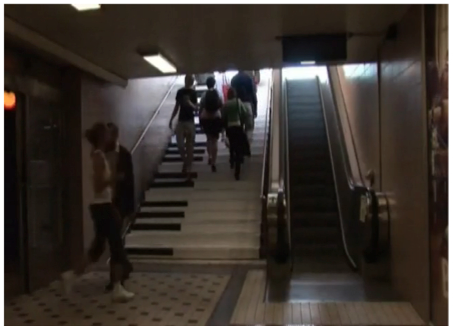
\includegraphics[width=9cm]{images/escada_gamificacao.png}
  \caption[Caso Volkswagem]{Exemplo do caso Volkswagem  - Teoria da Diversão (thefuntheory.com)}
  \label{fig:exampleFigPiano}
\end{center}
\end{figure}

	
De acordo com \cite{hagglund2012}, a maioria das pessoas gostam de jogar pelo menos algum tipo de jogo. Esconde-esconde, xadrez ou os mais recentes games de computador são exemplos de jogos que estão sendo jogados todos os dias. Não obstante, na vida cotidiana, essas pessoas precisam realizar tarefas estressantes ou que, simplesmente, não se sentem motivadas a fazerem. Com a introdução de elementos de jogos, essas atividades poderiam, também, se tornar divertidas, gratificantes e agradáveis, onde as pessoas iriam, possivelmente, querer participar dessas tarefas proativamente e de forma contínua. Para  \cite{hagglund2012}, esse processo caracteriza a  gamificação.  
	
Como exemplo, além do que já fora ilustrado na figura \figref{fig:exampleFigPiano}, a Gamificação aplicada a  educação  pode fazer com que os alunos sintam-se mais motivados a frequentarem as escolas, bem como corroborar o aprendizado. No trabalho, pode fazer com que os funcionários se sintam mais animados com o serviço de modo a aumentarem a produtividade.  Nos sistemas de crowdsoursing, essa técnica pode engajar e motivar as pessoas a executaram as tarefas, tornando essa ação cada vez mais frequente. Consequentemente, aumentando a capacidade de recrutamento e, sobretudo, melhorando a forma com que as tarefas são projetadas.          

Segundo \cite{pereira2011}, existem várias técnicas e artifícios de jogos que podem ser utilizados em uma gamificação. Embasado pelo trabalho feito por \cite{lands2011}, ele destaca as seguintes técnicas como as principais:

\begin{itemize}
\item \textbf{Medalhas e insígnias} – consiste na premiação por metas, através de medalhas que simbolizem a conquista, de modo que outras pessoas vejam o empenho do jogador e sinta-se motivado a ter o mesmo desempenho que este;
\item \textbf{Níveis} -  Atividades separadas por níveis para que o jogador fique ciente de qual nível ele esta e quanto ele falta para que possa evoluir;
\item \textbf{Rankings} – tem o objetivo de criar rivalidade e, consequentemente, aumentar o foco no objetivo. Pois, a ideia é que os jogadores competitivos sempre estarão em busca do primeiro lugar;
\item \textbf{Barra de Progresso} – estímulo visual de modo a mostrar ao usuário qual é o seu progresso diante ao objetivo final;
\item \textbf{Moeda Virtual} – consiste em disponibilizar moedas virtuais para que possam ser trocadas posteriormente por itens ou premiações reais.
\item \textbf{Sistemas de pontos} – uma vez que existem pontuações diferentes para atividades diferentes, o usuário perceberá que algumas atividades podem ser mais importantes que outras;
\item \textbf{Desafio entre os usuários} – permite que o usuário possa ser comparado a outro e buscar meios de vencê-lo;
\item \textbf{Bônus}: oferecer uma premiação extra para o usuário que consegue completar uma determinada tarefa;
\item \textbf{Colaboração em comunidade} – aumentar a interatividade entre os usuários;
\item \textbf{Pontuação por tempo} – acaba atribuindo um senso de urgência, fazendo com que os usuários priorizem determinadas tarefas.
\end{itemize}

Na proposta deste trabalho, a gamificação é utilizada como parte do processo de estímulo  a execução das tarefas de colaboração existente no sistema. Tais tarefas são explicadas detalhadamente no próximo capítulo.


\chapter{Trabalhos Relacionados}
\label{ch:trabalhosRelacionados}

Atualmente, existem diversos projetos para Smartphones que possuem algumas características semelhantes ao FindBus. Contundo, apesar de todas elas buscarem resolver o mesmo problema da falta de informação no tocante a serviços disponíveis do transporte público elas se diferem em diversos aspectos. 
	
Neste seção iremos descrever em detalhes as tecnologias, benefícios e, principalmente, funcionalidades das mais importantes aplicações em tempo real para o transporte público. Para tanto, esses sistemas foram selecionados de acordo com o campo de utilização (trem, avião, ônibus, metrô, carro, etc) e os parâmetros e características comuns entre eles e o projeto FindBus, tema deste trabalho. 

A seguir estão as aplicações em tempo real discutidas nesta seção:

\begin{itemize}

\item Waze
\item Moovit
\item Google Transit
\item TRIPGO
\item Triptastic
\item LONDONER PRO BUS \& TUBE
\item City \& Bus Napoli 
\item MuoviMi
\item Marretai
\end{itemize}

\section{Waze}

O Waze é uma aplicação que fornece ao usuário o conhecimento do estado atual do tráfego, permitindo que estes saibam em, praticamente, tempo real as condições das estradas, bem como a forma mais rápida de se chegar a um determinado destino. 

De acordo com [Waze 2011], a ferramenta consiste em um sistema de navegação baseado em informações de condições das estradas obtidas em tempo real, onde os dados utilizados são inteiramente fornecidos pelos usuários através de postagens realizadas pela interface do próprio aplicativo, tais postagens podem conter textos e imagens que podem ser tiradas na hora pelo próprio dispositivos, bem como caracteriza uma grande interação social entre os membros do aplicativo, por exemplo, se um usuário passa por um acidente, ele pode emitir um alerta para que outros membros possam ficar cientes deste incidente e, por ventura, troquem de rota. Ademais, a localização do usuário é fornecida a todo momento por meio de um receptor GPS presente no dispositivo móvel em que o aplicativo estiver instalado.   
 
No que se  refere a se comportar como um utilitário de GPS, o Waze fornece quase os mesmos recursos que outros aplicativos ou GPSs convencionais: navegação, guia por voz, tráfego e etc. Todavia, o mesmo possui diferenciais consideráveis, justamente, pelo fato de possuir uma intensa socialização entre os membros, segue abaixo alguns desses diferencias:

\begin{itemize}
\item Rotas de transito em tempo real baseadas nas informações do transito;
\item Alertas de acidentes emitidos pelos membros;
\item Alteração da rota quando as condições da via mudam;
\item Integração com Redes Sociais;
\item É possível ver seus amigos dirigindo para o mesmo local que você;
\item Ao navegar com o aplicativo ativo, você contribui para as informações que os outros membros poderão ver;
\item Evolução de seu perfil conforme você contribui para a melhor navegação de todos.
\end{itemize}

\begin{figure}[htp]
\begin{center}
  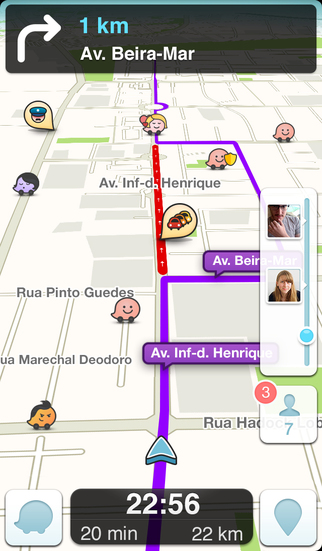
\includegraphics[width=5cm]{images/waze1.jpg}
    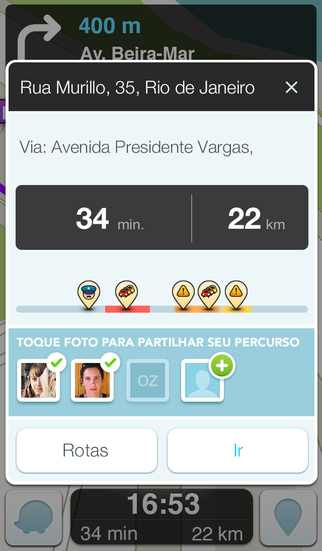
\includegraphics[width=5cm]{images/waze2.jpg}
  \caption{Exemplo do aplicativo Waze}
  \label{fig:exampleWaze}
\end{center}
\end{figure}

\section{Moovit}

O Moovit é um aplicativo de GPS mobile desenvolvido pela startup israelense Tranzmate, que consiste em fornecer informações referentes ao transporte público em tempo real, bem como navegação GPS em todos os modos de transporte, incluindo ônibus, trólebus, bondes, trens, metrôs e ferries. Para tanto, os usuários acessam um mapa ao vivo onde, além das informações citadas,  podem visualizar as paradas e estações de base próximas de acordo com sua localização GPS atual, bem como podem planejar viagens em todos os modos de transporte com base em dados em tempo real oriundos de outros membros do aplicativo.
	
\begin{figure}[htp]
\begin{center}
  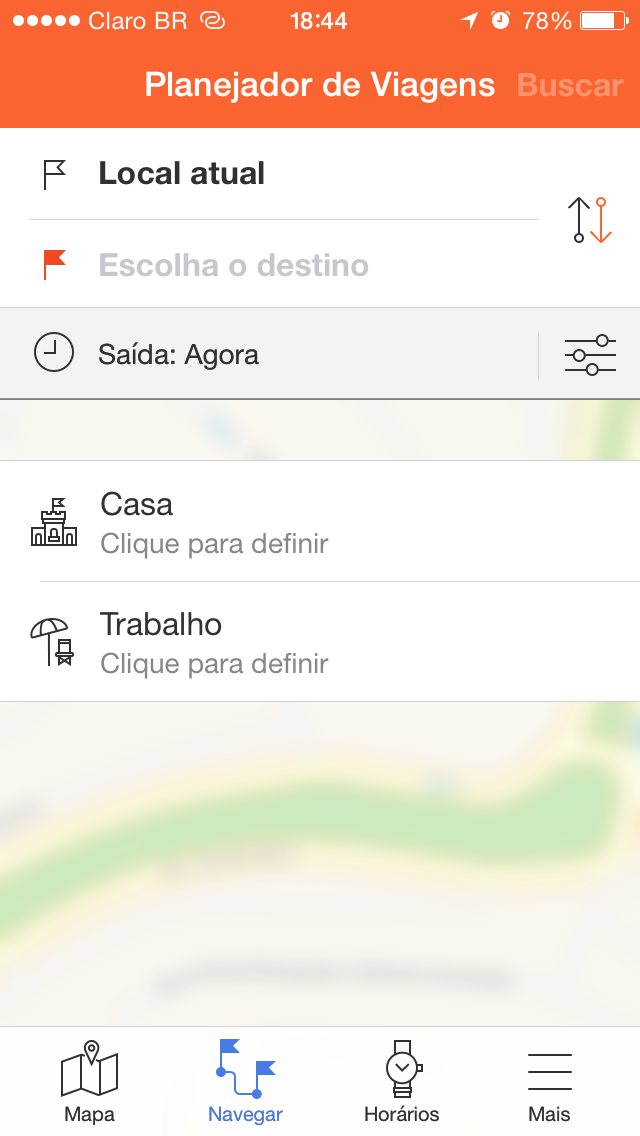
\includegraphics[width=5cm]{images/moovit1.png}
    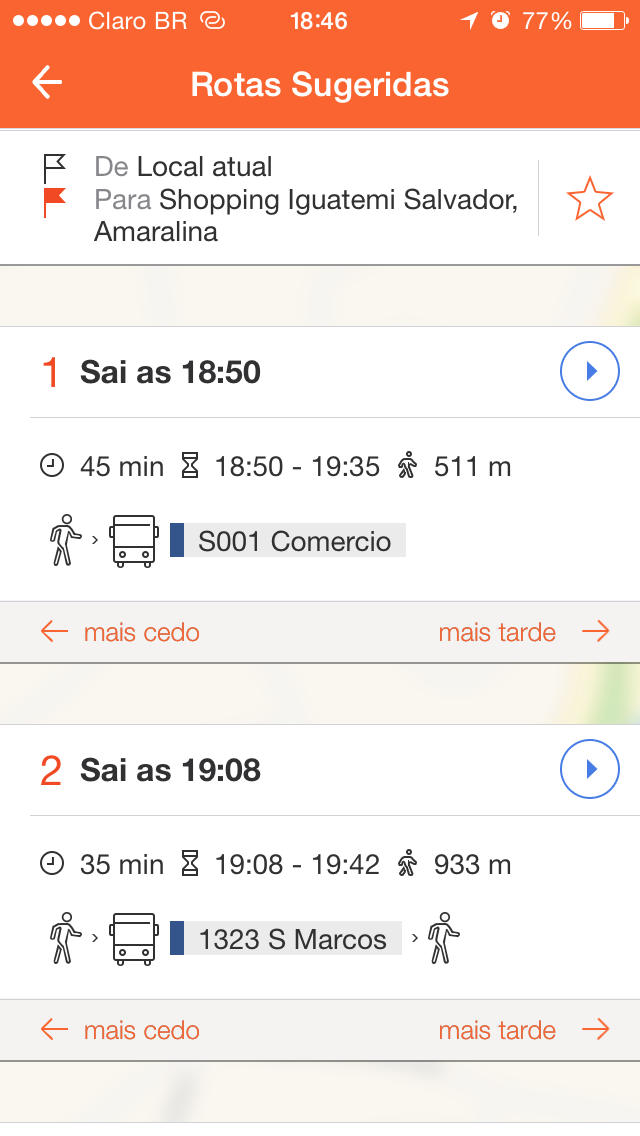
\includegraphics[width=5cm]{images/moovit2.png}
  \caption{Exemplo do aplicativo Moovit}
  \label{fig:exampleMoovit}
\end{center}
\end{figure}

Os dados disponibilizados pela aplicação difere das informações de transporte público tradicionais, pois é um aplicativo voltado para a comunidade que integra dados de transporte público estáticos a partir de operadores de trânsito com dados em tempo real coletados de usuários via crowdsourcing. Isso é possível pois os usuários somente por estarem com o aplicativo aberto fornecem, de forma passiva e anonimamente, os seus dados de velocidade e de localização para Moovit. A aplicação então integra esses dados obtidos através do uso de crowdsourcing com dados estáticos de horários de transporte público para melhorar os resultados do plano de viagem com base nas condições atuais das vias, e compartilhar esses dados com a comunidade de usuários. Além de compartilhar os dados passivamente, os usuários podem enviar ativamente alertas, incluindo razões para os atrasos, superlotação, a satisfação com o motorista do ônibus, e disponibilidade wi-fi nos terminais e meios de transporte.
	
Isto posto, resumidamente, o Moovit se propõe a ajudar o usuário a encontrar o melhor caminho para chegar a um determinado lugar através dos diversos meios de transportes públicos existentes, graças às informações fornecidas pela comunidade em tempo real. Segue abaixo algumas das principais características dessa aplicação: 

\begin{itemize}
\item Planejamento de rota - a comunidade notifica em tempo real a situação do transporte público,  bem como ajuda a identificar os meios de transporte  mais confortáveis para as necessidades do usuário. 
\item Reduzir o tempo de espera no ponto de ônibus – Permite que o usuário verifique o andamento de seu veículo em tempo real no mapa e, assim,  se desloque  para o ponto de ônibus, sem perder tempo. 
\item Informações sobre a hora prevista de chegada – tempo de chegada atualizado em tempo real durante a viagem. 
\item Alertas em tempo real fornecido pelos usuários - receber e enviar informação referentes a causas de atraso, situação de pontos de ônibus, linhas e pilotos. 
\item Navegação – interface de navegação que fornece ao usuário o mapa da cidade, bem como o  percurso a ser seguido. 
\item Em torno do usuário – ajudar o usuário a encontrar as paradas mais próximas de sua localização e visualizar as informações sobre horários de chegada e saída para as linhas que lhe interessam.
\end{itemize}

\section{Google Transit/Google Maps}

O Google Transit, que começou como um projeto do Google Labs em dezembro de 2005 e agora está integrado diretamente no produto Google Maps [wiki],  fornece ao usuário o planejamento de viagens em diversas cidades ao redor do mundo. Para tanto, interfaces para o Google Transit existem em uma variedade de dispositivos móveis, empregando sensores de localização, como GPS e Wi-Fi de localização no dispositivo para determinar um local de partida para o planejamento de uma viagem, bem como coletar informações como localização e velocidade do usuário. 	

\begin{figure}[htp]
\begin{center}
  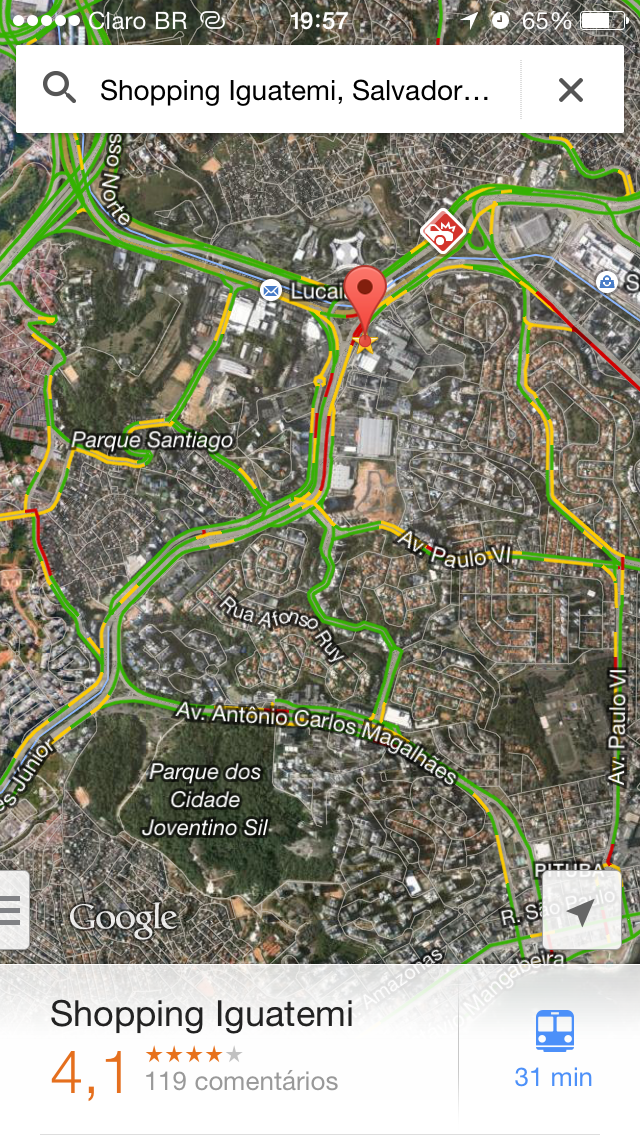
\includegraphics[width=5cm]{images/maps2.png}
    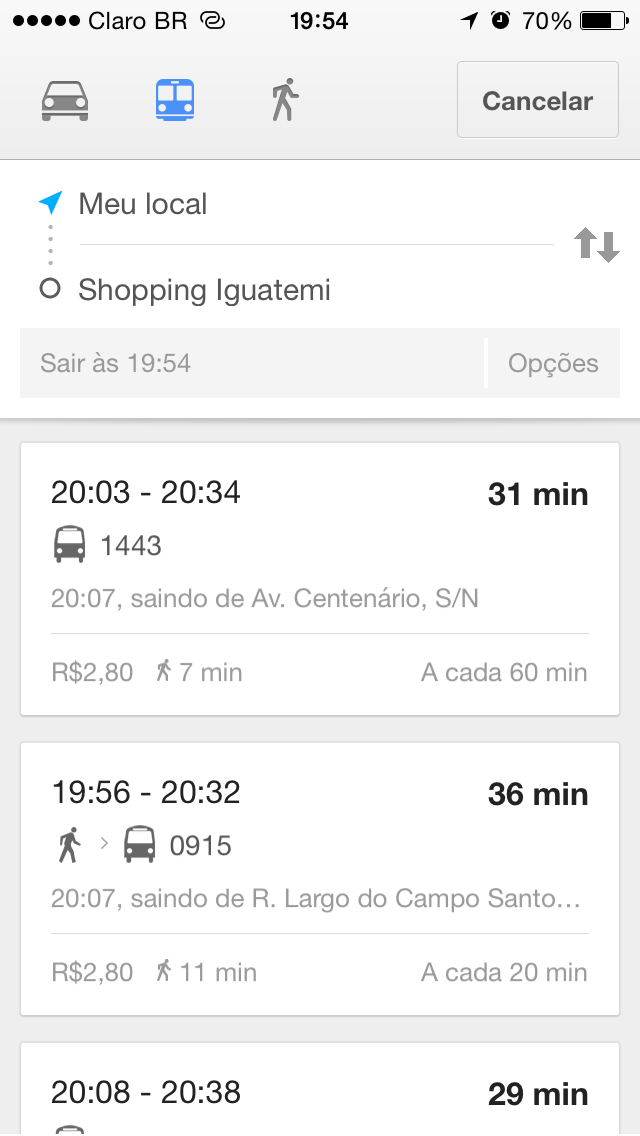
\includegraphics[width=5cm]{images/maps3.png}
  \caption{Exemplo do aplicativo Google Maps}
  \label{fig:exampleMaps}
\end{center}
\end{figure}

Ademais, o Google Maps informa as condições de trânsito nas principais vias de inúmeras cidades do planeta através de informações oriundas de autoridades de trânsito locais e, sobretudo, de dados dos próprios usuários. As informações que são coletadas, como posição e velocidade, são fornecidas pelos usuários de forma passiva e anônima quando estes estão utilizando o aplicativo. Deste modo, o Google Transit pode, em tempo real, informar as condições de tráfego das vias, bem como indicar o melhor caminho a ser seguido para se chegar a um determinado destino.

Nesse sentido, o Google Transit, conectado com o Google Maps, fornece ao usuário a possibilidade de receber informações, em tempo real e de acordo com a viagem planejada, a partir de informações fornecidas por outros membros e automaticamente atualizar o mapa e as estradas de acordo com os eventos ou alertas informados. 

\section{TripGo}

O TripGo mostra todas as opções de transporte para se deslocar de um ponto a outro em toda cidade de Sydney, permitindo que o usuário consiga, instantaneamente, ver como chegar a seus lugares favoritos usando o caminho mais rápido e, sobretudo, mais barato.

\begin{figure}[htp]
\begin{center}
  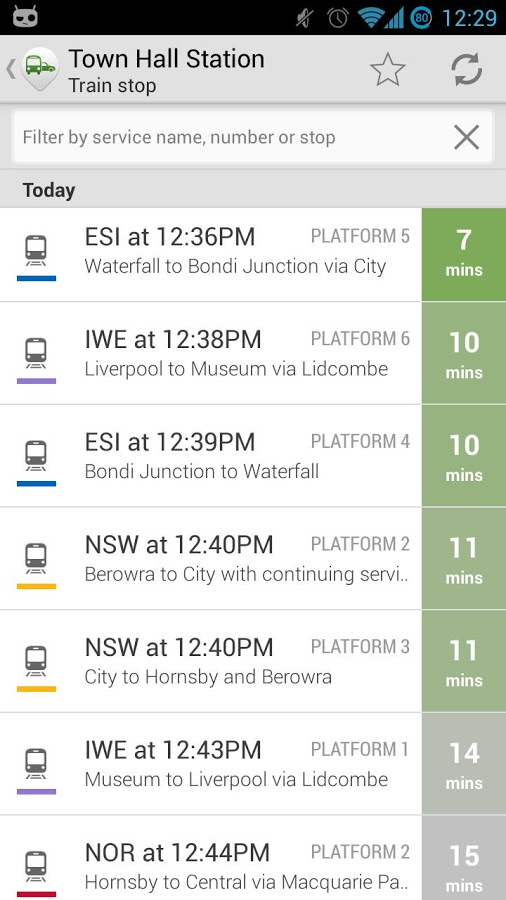
\includegraphics[width=5cm]{images/tripgo1.jpg}
    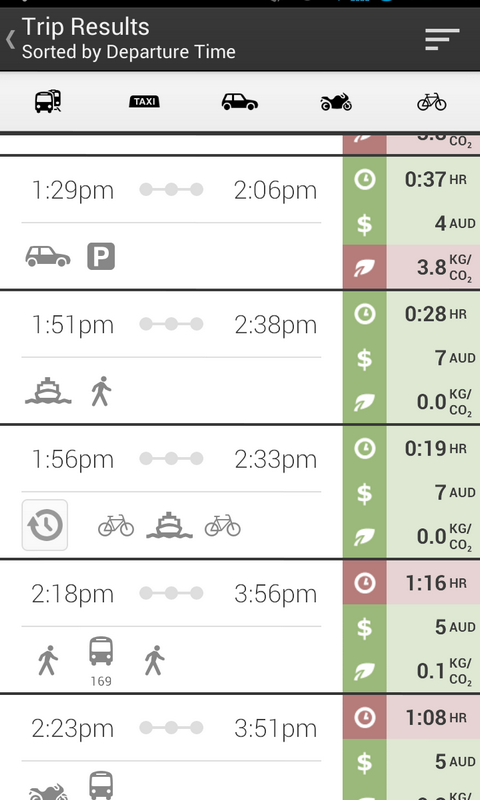
\includegraphics[width=5cm]{images/tripgo2.png}
  \caption{Exemplo do aplicativo TripGo}
  \label{fig:exampleTripGo}
\end{center}
\end{figure}

O usuário pode iniciar o planejamento de 2 maneiras:

\begin{enumerate}
\item Encontrar um caminho: Planejar uma viagem de um ponto a outro usando o transporte público, táxi, carro, moto, bicicleta, compartilhamento de bicicletas e caminhadas. Isto inclui combinações, como pegar um táxi para uma estação de trem e desta pegar um trem para outra estação.
\item Encontrar um serviço: Se o usuário já sabe o caminho, o mesmo pode utilizar o TripGo para encontrar um serviço, como por exemplo, os pontos mais próximos, os próximos horários, dentre outros.
\end{enumerate}

Segue abaixo alguns dos recursos fornecidos pelo TripGo:

\begin{itemize}
\item Disponibilizar informações de transporte público como horários de partida e de chegada previstos, localizações de GPS e alertas de serviço;
\item Permite o usuário adicionar seus destinos favoritos e obter acesso rápido a viagem para estes posteriormente;
\item Adicionar seus pontos de ônibus favoritos e manter seus filtros;
\item Adicionar um lembrete para uma viagem ou serviço para que o usuário seja notificado no exata momento que deva sair;
\item Informações detalhadas sobre o tempo e preço dos principais meios de transporte;
\item Permite que o usuário via o custo total de qualquer viagem, incluindo passagens, tarifa de táxi, potagens e tarifas de estacionamentos;
\item Mostra endereços e bares, restaurantes, lojas e outros pontos de interesse durante o percurso de uma viagem;
\item Planejar uma viagem futura, adicionando no calendário de viagens.
\end{itemize}

\section{Triptastic}

O Triptastic permite  que o usuário possa ver para onde pode ir a partir da sua localização atual e dos próximos serviços disponíveis que podem levá-lo até seu destino. Ademais, o usuário também pode explorar mapas detalhados e interativas que mostram  as rotas, paradas e frequências de serviços de transporte disponíveis no momento. 

O aplicativo fornece horários precisos e mapas para ônibus, trens e balsas em diversas cidades, por exemplo Sydney, Brisbane, Adelaide, Perth, Canberra, Newcastle, Wollongong, na Gold Coast, Queensland e Christchurch. 

As principais funcionalidades do TripTastic são:

\begin{itemize}
\item Em algumas cidades como  Sydney, Brisbane e Christchurch permite que o usuário acompanhe a real localização do ônibus enquanto o mesmo se desloca;
\item Explorar mapas dinâmicos em tempo real de rotas de trânsito, paradas e serviços disponíveis;
\item Não há necessidade de configurar viagens ou entrar com  pesquisas, pois com um toque na aplicação o usuário sabe onde ele pode ir e quando o próximo serviço chega;
\item Informações detalhadas a respeito dos veículos, se o mesmo tem ar-condicionado ou acessibilidade para cadeirantes, por exemplo;
\item Possui um motor de busca integrado para facilitar  a vida do usuário no que tange a encontrar rotas, pontos de ônibus, linhas e serviços. 
\end{itemize}

\begin{figure}[htp]
\begin{center}
  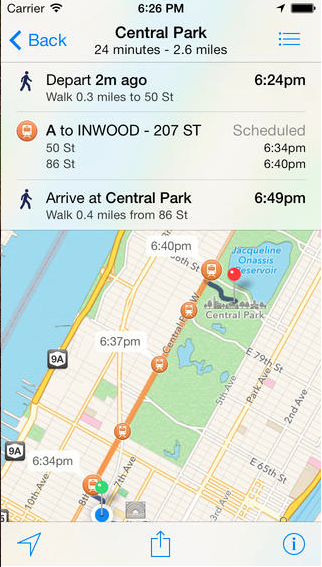
\includegraphics[width=5cm]{images/app1.png}
    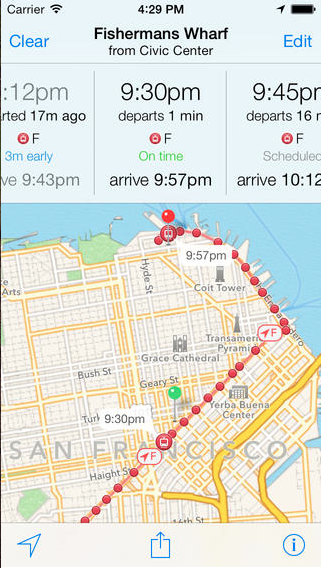
\includegraphics[width=5cm]{images/app2.png}
  \caption{Exemplo do aplicativo Triptastic}
  \label{fig:exampleTriptastic}
\end{center}
\end{figure}


\section{LONDONER PRO BUS \& TUBE}

Este aplicativo é o aplicativo mais importante de Londres no que tange a disponibilizar informações em tempo real sobre o transporte público [referencia]. Ele inclui todos os tipos de transporte público existente na capital, bem como informações de serviços de transporte disponíveis 24 horas e uma calculadora de preço estimado de viagem.

\begin{figure}[htp]
\begin{center}
  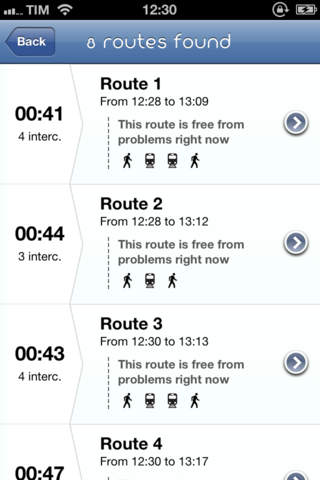
\includegraphics[width=5cm]{images/london1.jpg}
    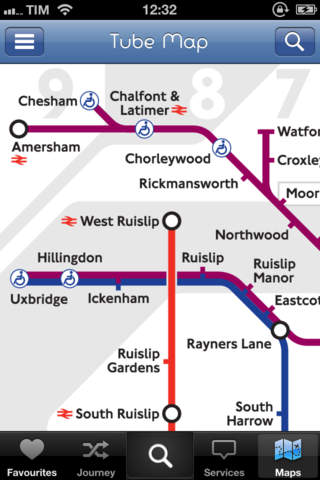
\includegraphics[width=5cm]{images/lodon2.jpg}
  \caption{Exemplo do aplicativo LONDONER PRO BUS \& TUBE}
  \label{fig:exampleLondon}
\end{center}
\end{figure}

Segue as principais características desta aplicação:

\begin{itemize}
\item Mostrar próximas paradas de um determinado ônibus;
\item Informar quais são os próximos ônibus que vão chegar em um ponto;
\item Guardar e organizar as linhas, pontos e ônibus favoritos;
\item Mostrar a rota completa de cada linha;
\item Buscar e salvar estações de ônibus, metrô, bicicleta e taxi favoritas;
\item Diversos recursos e configurações para planejamento de viagens ;
\item Mostrar serviços de taxi próximos e disponíveis;
\item Salvar o endereço, chamadas e serviços de taxis favoritos;
\item Planejar uma viagem combinando os diversos serviços de transporte disponíveis, bem como calcular o preço desta viagem;
\item Mostrar e planejar viagens utilizando as estações de bicicletas existentes, bem como mostrar todas informações relacionadas a essas estações, como preço, quantidade de bicicletas disponíveis ;
\item Mapa off-line 
\end{itemize}

O aplicativo também permite que o usuário configure as rotas e as salve para obter as informações off-line e permitir que os usuários tenham informações sobre a rota também em caso de ausência de rede.

\section{City \& Bus Napoli}

City \& Bus Napoli é um aplicativo desenvolvido pela LUSI-Lab, Laboratório de Informática do Departamento de Ciências Físicas da Universidade Federico II de Nápoles e permite que o usuário possa saber as rotas de ônibus, bondes e metrô em toda a cidade, bem como os principais pontos de interesse cultural na área e também saber em tempo real os tempos de chegada do transporte público (se e quando eles estão em circulação) a um determinado ponto ou estação. 

\begin{figure}[htp]
\begin{center}
  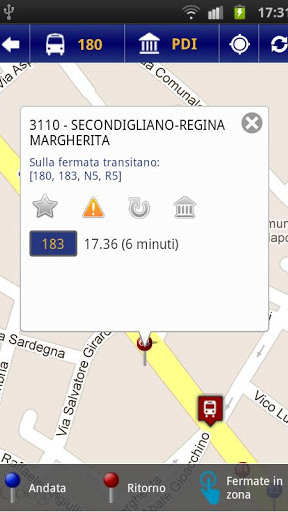
\includegraphics[width=5cm]{images/citybus.png}
    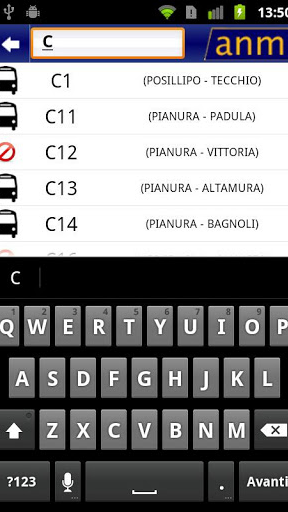
\includegraphics[width=5cm]{images/citybus2.png}
  \caption{Exemplo do aplicativo City \& Bus Napoli}
  \label{fig:exampleCity}
\end{center}
\end{figure}

As principais características desta aplicação estão a seguir listadas:

\begin{itemize}
\item Visualizar no aparelho um mapa com todas as paradas feitas por uma linha especial do transporte público de Napoli. 
\item Receber informações adicionais sobre uma parada ou linhas em trânsito, como possíveis desvios; 
\item Saber em tempo real a posição dos meios de transporte público disponíveis na cidade;
\item Informações detalhadas sobre um local turístico particular e como chegar até lá.
\end{itemize}

Além disso, o aplicativo permite visualizar informações sobre as atrações turísticas nas proximidades do usuário, organizados em categorias ou em áreas selecionadas.

\section{MuoviMi}

O MuoviMi é um aplicativo que torna mais fácil viajar de transportes públicos na cidade de Milão – Itália, fornecendo informações imediatas sobre horários de voos, linhas e tempos de espera de mais de 3.000 pontos de ônibus por toda a cidade, cerca de 150 linhas urbanas e interurbanas de superfície e de toda a rede subterrânea. Para tanto, o aplicativo requer uma conexão com a Internet para baixar as informações sobre horários e tempos de espera. 

As principais características são:

\begin{itemize}
\item Informações sobre mais de 4.000 pontos de ônibus em toda a cidade e província, com os tempos de espera (quando disponível) e horários programados;
\item Escolha dos pontos de ônibus favoritos para que usuário possa acessar facilmente todas as informações posteriormente;
\item Filtrar todas as linhas existentes para que se possa ter um acesso rápido a linha desejada;
\item Visualizar todos os pontos próximos;
\item Manter o controle dos horários programados em cache, para que o usuário possa acessá-los mesmo quando não tem uma conexão com a Internet.
\end{itemize}

\begin{figure}[htp]
\begin{center}
  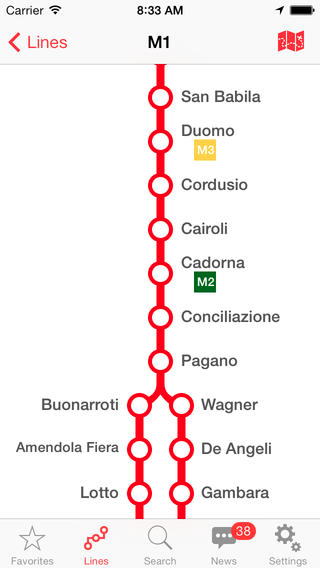
\includegraphics[width=5cm]{images/MuoviMI.png}
    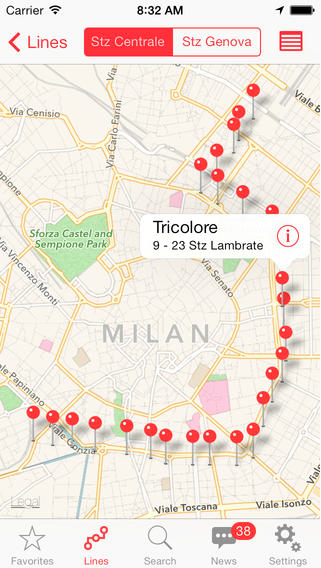
\includegraphics[width=5cm]{images/MuoviMI2.png}
  \caption{Exemplo do aplicativo MuoviMi}
  \label{fig:exampleMuoviMi}
\end{center}
\end{figure}

\section{Marsrutai}

Marsrutai é um aplicativo criado por desenvolvedores  lituanos e fora, inicialmente, projetado para a capital Vilnius e mais tarde alargado a muitas outras cidades do país. Ele permite o planejamento de uma viagem  especificando várias opções decididas pelo usuário. 

O aplicativo permite três tipos de pesquisa: 

\begin{itemize}
\item planejador típico de viagem pela inserção de um ponto de partida e de destino ;
\item busca de uma determinada estação na cidade selecionada; 
\item busca de uma rota específica com base na seleção de um meio de transporte público específico. 
\end{itemize}

O aplicativo também permite a recepção de dados sobre a posição, em tempo real,  do transporte selecionado, exibindo no mapa o seu caminho e notificando o usuário todas as informações sobre atrasos e problemas ao decorrer do percurso.

\begin{figure}[htp]
\begin{center}
  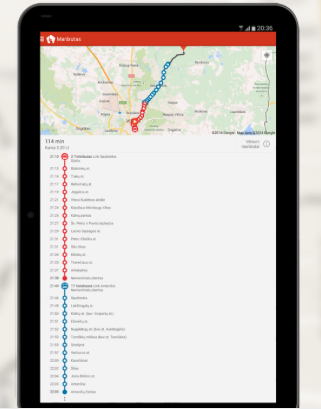
\includegraphics[width=5cm]{images/Marsrutai.png}
    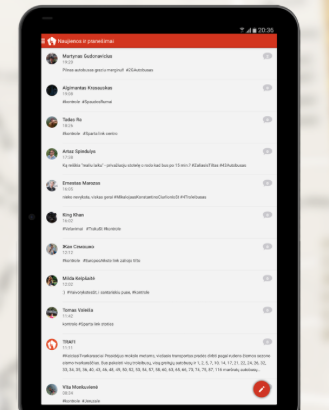
\includegraphics[width=5cm]{images/Marsrutai2.png}
  \caption{Exemplo do aplicativo Marsrutai}
  \label{fig:exampleMarsrutai}
\end{center}
\end{figure}

\section{Quadro Comparativo}

Esta subseção apresenta um quadro comparativo que visa comparar todas as aplicações encontradas durante a pesquisa de modo a ter uma visão mais detalhada de acordo com o:

\begin{itemize}
\item Tipo - o tipo de aplicação, em termos de área de desenvolvimento e do tipo de serviço de transporte público;
\item Serviço - a lista dos principais serviços oferecidos a partir dos aplicativos para os usuários:
\subitem Plataforma - tipos de plataformas em que o aplicativo é desenvolvido (web, mobile, etc ...);
\subitem Meios de Transporte -  Tipos de transportes públicos suportados;
\subitem Cidades -  Quantas cidades o aplicativo consegue fornecer o serviço;
\item A lista das principais funcionalidades oferecidas aos usuários para planejar, monitorar e controlar as suas viagens:
\subitem Planejamento - planejamento da viagem suportados;
\subitem Controle - gestão de eventos e possível re-plano da viagem (remostrar um novo caminho de acordo com os eventos recebidos);  
\item Gestão da informação - uma lista do tipo de informações tratadas e formatos suportados;
\subitem Dados abertos - dados abertos pelo governo local, instituições de trânsito ou fornecedores;
\subitem Dados de Crowdsourcing - dados coletados pelos usuários e seus dispositivos móveis; 
\subitem Dados sociais - dados recuperados pelas redes sociais e meios de comunicação social.
\end{itemize}

Segue abaixo a tabela que corresponde ao quadro comparativo descrito nesta seção:


\chapter{Proposta: Aplicativo FindBus}
\label{ch:finsbus}

\section{Proposta Metodológica}
\label{sc:propostaMetodologica}

Os processos de software são complexos e não existe um processo ideal que atenda a todos os sistemas. A maioria das empresas acaba desenvolvendo seus próprios processos de desenvolvimento de software com base em processos existentes, acrescentando ou retirando fases \citep{SOMMERVILLE2011}. A metodologia seguida neste projeto utiliza na sua primeira fase o encadeamento do modelo em cascata, com a inserção de incrementos do modelo incremental na sua segunda fase. Além disso, houve o acréscimo de uma atividade, chamada de Aprofundamento Teórico na primeira fase, conforme pode ser visto na figura \figref{fig:exampleMetodologia}.

\begin{figure}[htp]
\begin{center}
  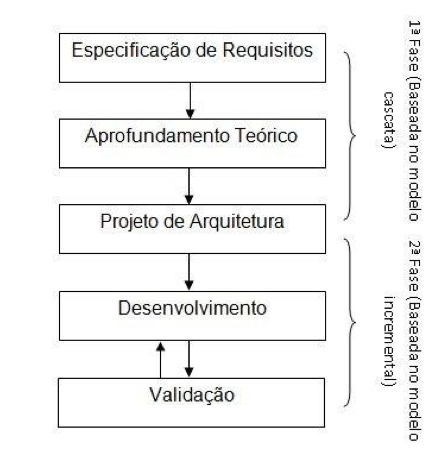
\includegraphics[width=7cm]{images/metodologia.png}
  \caption{Etapas da Metodologia do Projeto}
  \label{fig:exampleMetodologia}
\end{center}
\end{figure}

A primeira fase é composta por três atividades básicas: Especificação de Requisitos, Aprofundamento Teórico e Projeto de Arquitetura.

Na atividade de Especificação de Requisitos, os serviços, restrições e metas do sistema foram estabelecidas com base nas necessidades dos usuários. Esta atividade é apresentada na seção \ref{sc:EspecificacaoRequisitos}. Após o levantamento de requisitos foram produzidos dois diagramas para ajudar a modelagem da arquitetura: o diagrama de casos de usos, descrito na seção \ref{sc:casosDeUso} e, o diagrama de sequência, descrito na seção \ref{sc:diagramaDeSequencia} . Na atividade de Aprofundamento Teórico, foram estudados trabalhos que apresentavam características semelhantes a proposta deste trabalho. O resultado desta pesquisa foi descrita no capítulo \ref{ch:trabalhosRelacionados}.

A primeira fase desta metodologia, se baseia na rigidez necessária do modelo em cascata, onde cada atividade não é iniciada até que a atividade anterior esteja finalizada. Como o projeto de uma arquitetura precisa levar em consideração todos (ou a maioria) os seus componentes e interações entre eles, as atividades de Especificação de Requisitos e Aprofundamento Teórico tiveram que ser finalizadas antes que a atividade de Projeto de Arquitetura pudesse ser iniciada. Nesta atividade, com base nos resultados obtidos das duas atividades anteriores, foi produzido um modelo genérico de arquitetura que atende os requisitos levantados e que possui os componentes principais para o desenvolvimento da aplicação mobile sensível ao contexto de apoio ao transporte público, possível de ser implementada em diversas plataformas móveis. O modelo de arquitetura produzido nesta atividade pode ser visto em mais detalhes na seção \ref{sc:arquitetura}.

A segunda fase, inspirada no modelo incremental, contém as atividades de Desenvolvimento e Validação.

Nesta fase, pequenos incrementos, ou seja, pequenas versões do sistema eram produzidas e submetidas à validação. A estratégia foi escolher os componentes críticos da arquitetura, desenvolver pequenos aplicativos com estas funcionalidades, validá-los e depois agregar estas funcionalidades no aplicativo principal.

As plataformas de desenvolvimento escolhidas para a atividade de Desenvolvimento foram as plataformas Android da Google e IOS da Apple. Estas plataformas possibilitam o acesso e um controle quase que total aos recursos dos dispositivos de forma simples e factível. Por fim, a atividade de validação, apresentada também no capítulo \ref{ch:avaliacao}, verifica se o aplicativo FindBus, realmente, atende aos requisitos especificados na próxima sução.

\section{Especificação de Requisitos}
\label{sc:EspecificacaoRequisitos}

A especificação de software, também chamado de engenharia de requisitos, é um processo que envolve a compreensão e definição dos requisitos do sistema e identifica suas restrições referentes ao uso e desenvolvimento \citep{SOMMERVILLE2011}. O principal objetivo dessa fase é coletar, através da observação do ambiente do usuário, de outros sistemas existentes (manuais ou informatizados), da reutilização de análises anteriores, da leitura de obras de referências, de entrevistas com potências usuários, etc. os requisitos do problema a ser resolvido.

Entende-se por requisitos, as condições (o que o sistema deve fazer quais serviços oferecidos, restrições, etc.) que devem ser atendidas por um sistema ou parte dele, para satisfazer as necessidades dos usuários \citep{bezerra2007}.

Requisitos de software frequentemente recebem duas classificações \citep{SOMMERVILLE2011}: requisitos funcionais e requisitos não funcionais.

Os requisitos funcionais definem recursos específicos a serem fornecidos pelo sistema, o que ele deve fazer, como deve reagir a entradas específicas e seu comportamento em determinada situação, também dependem do tipo de software a ser desenvolvido, possíveis usuários, etc. A especificação dos requisitos funcionais de um sistema deve ser completa (os serviços requeridos pelo usuário devem ser definidos) e consistente (sem definições contraditórias) para evitar interpretações divergentes. Geralmente estes requisitos aplicam-se a características individuais ou serviços específicos do sistema.

Já os requisitos não funcionais, declaram as características de qualidade que o sistema deve possuir e que estão relacionadas as suas funcionalidades e, ao contrário dos requisitos funcionais, aplicam-se ao sistema como um todo. Podem afetar a arquitetura geral do sistema e podem gerar uma série de requisitos funcionais. Exemplos de requisitos não funcionais são: Confiabilidade (tempo entre falhas, recuperação de falhas, etc.), Desempenho (tempo de resposta esperado), Portabilidade (plataformas de hardware e software que o sistema será implantado, grau de facilidade para transportar o sistema para outra plataforma, etc.), Usabilidade (facilidade de uso, necessidade de treinamento, etc.), etc.

Os requisitos devem ser escritos em diferentes níveis de detalhamento, pois eles refletem informações sobre o sistema, para que diferentes leitores possam utilizá-los de diversas maneiras.

Esta seção especifica os requisitos do modelo de arquitetura proposto, fornecendo informações necessárias para o projeto e implementação, bem como para a realização dos testes.

Para a identificação dos requisitos foram adotadas as seguintes convenções: [RF00X] para requisitos funcionais; [RNF00X] para requisitos não funcionais; e [RI00X]  para requisitos de interface com o usuário.

Aos requisitos também foram atribuídas prioridades. Estas prioridades servem para indicar a relevância do requisito para a arquitetura proposta, que são elas: Essencial, são requisitos que precisam ser implementados impreterivelmente, indicando que sem tal requisito o sistema não entra em funcionamento ou não atende aos objetivos do trabalho proposto. Importante, são requisitos que o sistema entrará em funcionamento, porém, de forma parcial. Sendo que estes  devem ser implementados, mas se não forem, o sistema poderá ser usado. Desejável, são requisitos que não comprometem o funcionamento básico do sistema e que podem ser deixados para versões posteriores deste trabalho.

\subsection{Requisitos Funcionais}

A tabela abaixo apresenta os requisitos funcionais do sistema.


\begin{center}
\begin{longtable}{c|c|p{8cm}|c}
\hline
\textbf{Cod.} & \textbf{Nome} & \textbf{Descrição} & \textbf{Prioridade} \\
\hline
RF01  & Cadastro de Usuário & Permitir que o usuário possa realizar cadastro no sistema. & Essencial \\
\hline
    RF02  & Fazer Login & Permitir que um usuário tenha acesso às informações e funcionalidades do sistema. & Essencial \\
\hline
    RF03  & Fazer logoff & Permitir que o usuário saia do sistema. & Essencial \\
\hline
    RF04  & Encaixar no Contexto & Fazer com que os usuários sejam encaixados no contexto de sua cidade, assim, visualizando informações no tocante ao transporte público da mesma. & Importante \\
\hline
    RF05  & Mudança de Contexto & Permitir que o usuário mude para o contexto de outra cidade, desta forma, visualizando informações do transporte público da cidade escolhida. & Importante \\
\hline
    RF06  & Localização do Usuário & Permitir que o usuário visualize sua localização no mapa. & Importante \\
\hline
    RF07  & Localização dos ônibus & Permitir que o usuário saiba a localização de todos os ônibus que possui GPS. & Essencial \\
\hline
    RF08  & Deslocamento dos ônibus & Fazer com o usuário possa acompanhar o deslocamento dos ônibus em, praticamente, tempo real. & Essencial \\
\hline
    RF09  & Tempo de Atualização & Mostrar quanto tempo se passou desde a última atualização de um determinado ônibus. & Essencial \\
\hline
    RF10  & Localização dos Pontos & Permitir que o usuário visualize a localização de todos os pontos de ônibus do contexto em que ele se encontra. & Essencial \\
\hline
    RF11  & Linhas Existentes & Mostrar todas as linhas de ônibus existentes no contexto que o usuário se encontra. & Importante \\
\hline
    RF12  & Linhas X Pontos & Permitir que o usuário saiba quais linhas passam por um determinado ponto. & Importante \\
\hline
    RF13  & Linhas Favoritas & Permitir que o usuário possa escolher linhas como favoritas. & Desejável \\
\hline
    RF14  & Alerta de Proximidade & Permitir que o usuário escolha, das linhas favoritadas, quais linhas ele deseja receber uma notificação quando algum ônibus desta estiver se aproximando. & Desejável \\
\hline
    RF15  & Cadastro de Ocorrências & Permitir que o usuário possa informar os incidentes que estão acontecendo no trânsito. & Essencial \\
\hline
    RF16  & Detalhar Ocorrência & Dar ao usuário a possibilidade de detalhar a ocorrência com foto e uma descrição sobre a mesma. & Importante \\
\hline
    RF17  & Localização de Ocorrências & Mostrar a localização de todas as ocorrências existente no contexto que o usuário se encontra.   & Essencial \\
\hline
    RF18  & Linhas Afetadas & Permitir que o usuário saiba quais linhas estão sendo afetadas por uma determinada ocorrência. & Importante \\
\hline
    RF19  & Visualizar Ocorrência & Permitir que o usuário possa visualizar detalhes das ocorrências cadastradas pelas pessoas que estão vivenciando o problema. & Essencial \\
\hline
    RF20  & Monitoramento & Permitir que o usuário escolha uma linha de ônibus para monitorar e, desta forma, saber tudo que o sistema dispõe a respeito dela. & Importante \\
\hline
    RF21  & Mostrar trajeto & Mostrar, no mapa, todo trajeto de uma linha que está sendo monitorada. & Desejável \\
\hline
    RF22  & Recomendação de Linha & Recomendar a melhor linha de ônibus, no momento, para se chegar a um determinado destino fornecido pelo usuário. & Essencial \\
    \hline
    RF23  & Informações de Distância & Mostrar a distância existente entre um usuário e um ônibus, um ponto e uma ocorrência, bem como de uma determinada ocorrência para um ônibus escolhido pelo usuário. & Desejável \\
\hline
    RF24  & Informações de Endereço & Mostrar o endereço de todos os ícones existentes no mapa (ônibus, pontos, ocorrências e etc). & Desejável \\
\hline
   RF25 & Quantidade de ônibus & Mostrar ao usuários quantos ônibus estão rodando para uma determinada linha no momento. & Desejável\\
   \hline
    RF26 & Recuperação de Senha & O sistema deve permitir que o usuário recupere sua senha em caso de esquecimento. & Essencial\\
\hline
\caption{Requisitos funcionais do sistema}
\end{longtable}
\end{center}


\subsection{Requisitos Não Funcionais}

A tabela que segue apresenta os requisitos não funcionais do sistema classificados por suas características e subcaracterísticas.

\begin{center}
\begin{longtable}{c|p{11cm}|c}
\hline
    \multicolumn{3}{c}{\textbf{Funcionalidade}} \\
    \hline
    \textbf{Nome} & \textbf{Descrição} & \textbf{Subcaracterística} \\
    \hline
    RNF01 & O sistema deve demorar, no máximo, 2 minutos para atualizar a localização de um ônibus. & Acurácia  \\
    \hline
    RNF02 & O usuário deve receber a notificação de proximidade quando o ônibus entrar no raio de 1km de distância. & Acurácia  \\
    \hline
    RNF03 & Quando o veículo entrar no raio de 1km de distância do usuário, o sistema não deve demorar mais de 20 segundos para notificá-lo.  & Acurácia  \\
    \hline
    RNF04 & O sistema deve atualizar, todos os dias, as informações de linhas, rotas, pontos de ônibus e horários presentes no aplicativo. & Acurácia  \\
    \hline
    RNF05 & As informações referentes a localização dos ônibus no Banco de Dados devem ser atualizadas a cada 15 segundos. & Acurácia  \\
    \hline
    RNF06 & O sistema deverá interagir com servidores web através de WebService. & Interoperabilidade  \\
    \hline
    \multicolumn{3}{c}{\textbf{Usabilidade}} \\
    \hline
    \textbf{Nome} & \textbf{Descrição} & \textbf{Subcaracterística} \\
    \hline
    RNF07 & O sistema deve ser fácil e simples de usar sem a necessidade de manuais ou treinamento.  & Apreensibilidade  \\
    \hline
    RNF08 & O sistema deve exigir pouca interação explícita do usuário.  & Operacionalidade  \\
    \hline
    \multicolumn{3}{c}{\textbf{Portabilidade}} \\
    \hline
    \textbf{Nome} & \textbf{Descrição} & \textbf{Subcaracterística} \\
    \hline
    RNF09 & O sistema deve ser projetado de tal forma a poder ser desenvolvido em qualquer plataforma móvel, com poucas modificações.  & Adaptabilidade  \\
\hline
\caption{Requisitos não funcionais do sistema}
\end{longtable}
\end{center}

\subsection{Requisitos de Interface}

A tabela abaixo apresenta os requisitos de interface do sistema.

\begin{center}
\begin{longtable}{c|c|p{8cm}|c}
\hline
    \multicolumn{1}{c}{\textbf{Cod.}} & \multicolumn{1}{c}{\textbf{Nome}} & \multicolumn{1}{c}{\textbf{Descrição}} & \textbf{Prioridade} \\
\hline
    RI01  & Tela Principal & O sistema deve exibir, como tela principal, uma tela que contenha um mapa e informações dos ônibus e ocorrências encontradas na região.  & Essencial \\
    \hline
    RI02  & Caixa de Informação & Todas as caixas de informação de ícones, presente nos mapas apresentados no sistema, devem possuir o mesmo padrão. & Importante \\
    \hline
\caption{Requisitos de interface do sistema}
\end{longtable}
\end{center}

\subsection{Método para extração de Requisitos}

Para a extração dos requisitos, o método utilizado foi o método da conversação, pois fornece um meio de comunicação verbal entre duas ou mais pessoas, fornecendo uma forma eficaz dos usuários expressarem suas necessidades e responder às perguntas. Desta forma, foi realizada uma pesquisa com potenciais usuários do sistema  e visitas a estações de ônibus com o intuito de entender o funcionamento em comum dos mesmos.

\section{Arquitetura do Sistema}
\label{sc:arquitetura}

Arquitetura de software, segundo [Len Bass and Kazman (1997)], é a estrutura que abrange os componentes do sistema, as propriedades externas desses componentes, bem como as relações entre estes. Isto é, entende-se como arquitetura de software uma representação, em alto nível de abstração, que seja capaz de propiciar uma visão completa do sistema. Em outras palavras, a arquitetura de software consegue definir todos os componentes de software, suas propriedades e os relacionamentos existentes com outros sistemas. Analogamente, de acordo com [Garlan and Perry (1995)], a arquitetura de software é a estrutura dos componentes existentes em um sistema, suas inter-relações, bem como os fundamentos que regem seu entendimento e a evolução ao longo do tempo.

De acordo com \cite{SOMMERVILLE2011}, os conceitos de separação e independência são indispensáveis para o projeto de arquitetura, pois permitem que alterações sejam facilmente localizadas. Considerando a proposta deste trabalho, onde podem ocorrer diversas alterações, como inclusão de novas funcionalidades, bem como novas cidades, sobretudo, com certa frequência, tais conceitos são de suma importância. Assim sendo, a aplicação proposta foi modelada seguindo o padrão Model View Controller(MVC) que,  de acordo com \cite{SOMMERVILLE2011}, tem como objetivo separar os elementos de um sistema, permitindo que estes possam ser modificados de forma independente. Outrossim, essa independência nos possibilita alterar uma tela ou funcionalidade previamente existente, sem que haja a necessidade de quaisquer alterações nos dados subjacentes ao modelo, por exemplo.

No padrão MVC o sistema é estruturado em três componentes lógicos que interagem entre si: modelo, visão e controlador.

\begin{enumerate}
\item \textbf{Componente Modelo}: Gerencia o sistema de dados e as operações que estão associadas a estes dados.
\item \textbf{Componente Visão}: Define e gerencia como os dados são apresentados ao usuário.
\item \textbf{Componente Controlador}: Gerencia a interação do usuário (por exemplo, teclas, cliques do mouse etc.) e passa essas interações para a camada de Visão e o Modelo.
\end{enumerate}

Levando em consideração as definições e características do padrão MVC, a Figura ~\ref{fig:arquitetura} ilustra a arquitetura do sistema desenvolvido como proposta deste trabalho.
 
\begin{figure}[htp]
\begin{center}
  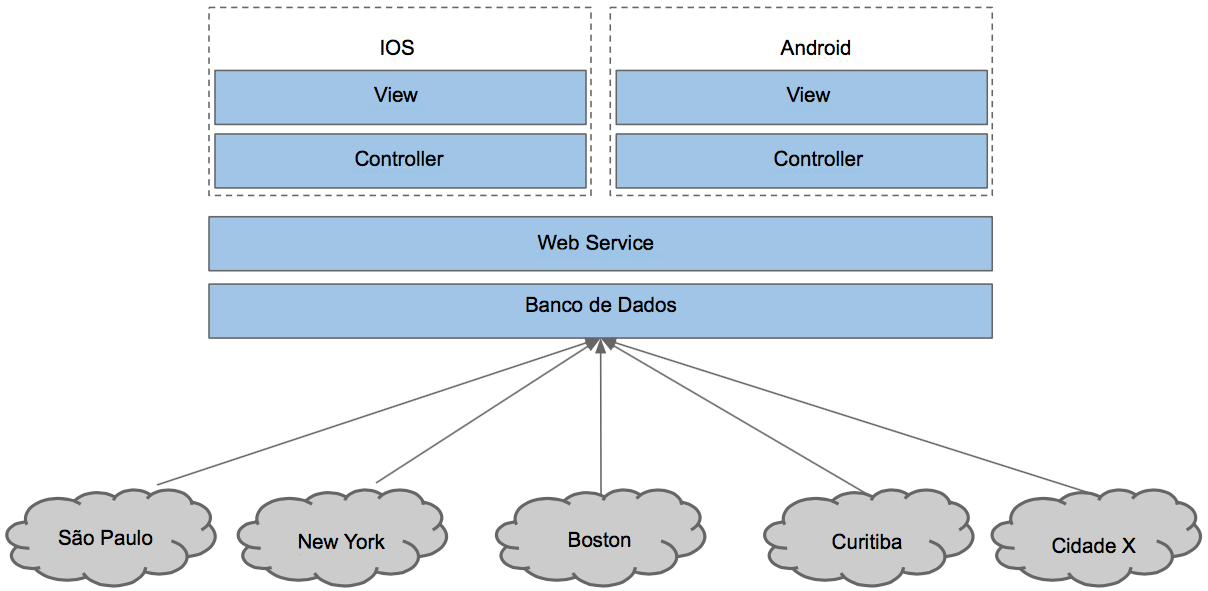
\includegraphics[width=17cm]{images/arquitetura.png}
  \caption{Arquitetura do trabalho proposto}
  \label{fig:arquitetura}
\end{center}
\end{figure}

As próximas subseções tem o objetivo de apresentar e explicar cada camada presente nesta arquitetura.  


\subsection{Composição da Arquitetura}
Nesta subse\c{c}\~{a}o ser\~{a}o descritos todos os componentes presentes na arquitetura proposta, mostrando a fun\c{c}\~{a}o de cada um dentro da arquitetura, seus pontos de extensibilidade, bem como sua intera\c{c}\~{a}o com elementos externos de forma a facilitar o desenvolvimento de uma aplica\c{c}\~{a}o m\'{o}vel sens\'{i}vel ao contexto, independente da plataforma de programa\c{c}\~{a}o utilizada.

\subsubsection{Camada View}
A camada de vis\~{a}o cont\'{e}m as telas que mant\'{e}m a intera\c{c}\~{a}o com o usu\'{a}rio. Esta camada \'{e} a respons\'{a}vel por enviar os eventos do usu\'{a}rio para a camada controller, onde os eventos ser\~{a}o tratados e o fluxo seguinte da aplica\c{c}\~{a}o ser\'{a} selecionado. Os detalhes de cada tela ser\~{a}o descritos na Se\c{c}\~{a}o~\ref{sc:telas}

\subsubsection{Camada Controller}
Elemento central da arquitetura. Tem a responsabilidade de coordenar o fluxo da aplica\c{c}\~{a}o e fazer a integra\c{c}\~{a}o entre as demais camadas. Respons\'{a}vel, tamb\'{e}m, por receber o processamento de um determinado componente e, com base no fluxo da aplica\c{c}\~{a}o, chamar o componente subsequente para dar continuidade ao processamento. Verifica novas informa\c{c}\~{o}es dos \^{o}nibus, atrav\'{e}s de web services, e atualiza a tela com as novas informa\c{c}\~{o}es.

\subsubsection{Camada Web Service}
Nesta camada est\c{c}o contidos todos os web services utilizados na aplica\c{c}\c{c}o. Os web services s\c{c}o componentes que permitem \`{a}s aplica\c{c}\~{o}es enviar e receber dados em diversos formatos como por exemplo XML e JSON. Esta camada tamb\'{e}m \'{e} respons\'{a}vel por permitir que novas aplica\c{c}\~{o}es interajam com as aplica\c{c}\~{o}es j\'{a} existentes e, tamb\'{e}m, garante a compatibilidade de sistemas desenvolvidos em plataformas diferentes.

\subsubsection{Camada Banco de Dados}
Camada de persist\^{e}ncia de dados que cont\'{e}m as regras de acesso \`{a} base de dados e demais fontes de armazenamento de informa\c{c}\~{o}es do sistema.\newline

As nuvens existentes na arquitetura representam outros sistemas externos que fornecem os dados das cidades monitorada pelo aplicativo. Ao passo que uma nova cidade \'{e} acrescentada, seus dados s\c{c}o armazenados na base de dados e, a partir da\'{i}, frequentemente atualizados. Isto possibilita que o acesso aos dados de diferentes sistemas seja feito de forma singular.



\section{Casos de Uso}
\label{sc:casosDeUso}

Os casos de uso são representações das funcionalidades de um sistema, percebidos por um observador externo a ele, ou seja, são as funcionalidades externas de um sistema e, como esse sistema interage com o ambiente externo \citep{bezerra07}. Os casos de uso s\~{a}o uma t\'{e}cnica para a descoberta de requisitos que foi introduzia inicialmente no m\'{e}todo Objectory \cite{jacobson93}. Atualmente os casos de uso s\~{a}o uma caracter\'{i}stica fundamental da linguagem de modelagem unificada(UML - do ingl\^{e}s unified modeling language). De acordo com \cite{SOMMERVILLE2011} os casos de uso, em sua forma mais simples, s\~{a}o capazes de identificar os atores envolvidos em uma intera\c{c}\~{a}o com o sistema, dando nome ao tipo da intera\c{c}\~{a}o. Ainda segundo \cite{SOMMERVILLE2011}, \`{a}s intera\c{c}\~{o}es s\~{a}o adicionadas algumas informa\c{c}\~{o}es que detalham a intera\c{c}\~{a}o com o sistema. Essa informa\c{c}\~{a}o adicional pode ser descrita textualmente ou representada por um ou diversos modelos gr\'{a}ficos como diagramas ou estados da UML.\newline

\begin{figure}[htp]
\begin{center}
  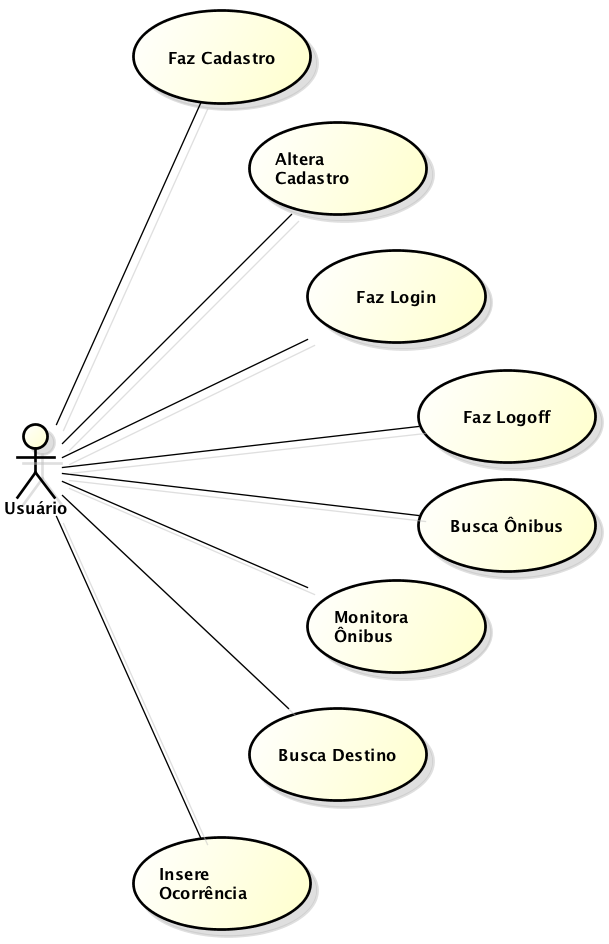
\includegraphics[width=11cm,height=10cm]{images/Diagramas/CasosDeUso_Geral.png}
  \caption{Diagrama de Casos de Uso - Geral}
  \label{fig:diagramaCasosDeUso}
\end{center}
\end{figure}

Casos de uso s\~{a}o documentados atrav\'{e}s de um diagrama de casos de uso de alto n\'{i}vel. O conjunto dos casos de uso representa todas as intera\c{c}\~{o}es poss\'{i}veis descritas nos requisitos do sistema.

De acordo com \cite{SOMMERVILLE2011}, n\~{a}o existe uma distin\c{c}\~{a}o entre cen\'{a}rios e casos de uso que seja simples e r\'{a}pida. A maioria das pessoas consideram cada caso de uso como sendo um cen\'{a}rio \'{u}nico. Contudo, autores em \cite{stevens06} sugeriram o encapsulamento do conjunto de cen\'{a}rios em um \'{u}nico caso de uso.

Os casos de uso identificam as intera\c{c}\~{o}es entre o sistema e seus usu\'{a}rios, ou outros sistemas, de forma individual. Acrescentando-se aos diagramas de casos de uso, dever\'{a} existir um documento com uma descri\c{c}\~{a}o textual para cada um deles.\newline

Considerando a elicita\c{c}\~{a}o de requisitos dos que v\~{a}o interagir diretamente com o sistema, os cen\'{a}rios e os casos de uso s\~{a}o t\'{e}cnicas bastante eficazes. Contudo, pelo fato dos casos de uso focarem na intera\c{c}\~{a}o com o sistema, eles n\~{a}o s\~{a}o t\~{a}o eficientes para elicitar requisitos n\~{a}o funcionais.

O diagrama de casos de uso geral est\'{a} representado na Figura~\ref{fig:diagramaCasosDeUso}. A representa\c{c}\~{a}o textual dos casos de uso considerados mais importantes ser\'{a} detalhada nas subse\c{c}\~{o}es seguintes.




\subsection{Caso de Uso 01 - Cadastrar Usu\'{a}rio}

\begin{center}
\begin{longtable}{p{8cm}|p{8cm}}
    \hline
    \textbf{Ator Principal} & Usu\'{a}rio \\
    \hline
    \textbf{Atores Secund\'{a}rios} & ------- \\
    \hline
    \textbf{Resumo} &  O usu\'{a}rio far\'{a} seu cadastro no sistema\\
    \hline
    \textbf{Pr\'{e}-condi\c{c}\~{o}es} & Usu\'{a}rio estar conectado \`{a} Internet\\
    \hline
    \textbf{P\'{o}s-condi\c{c}\~{o}es} & ------- \\
    \hline
    \hline
    \textbf{A\c{c}\~{o}es do Ator} & \textbf{A\c{c}\~{o}es do Sistema} \\
    \hline
    1. Seleciona bot\~{a}o "Cadastre-se" na tela de login & \\
    \hline
    2. Preenche os campos requisitados & \\
    \hline
    3. Seleciona bot\~{a}o para submeter os dados & \\
    \hline
    & 4. Envia os dados via web-service \\
    \hline
    & 5. Efetua o cadastro \\
    \hline
    \hline
    \textbf{Restri\c{c}\~{o}es/Valida\c{c}\~{o}es} & -------\\
\hline
\caption{Caso de Uso 01 - Cadastrar Usu\'{a}rio}
\end{longtable}
\end{center}

\subsection{Caso de Uso 02 - Inserir Ocorr\^{e}ncia}
\begin{center}
\begin{longtable}{p{8cm}|p{8cm}}
    \hline
    \textbf{Ator Principal} & Usu\'{a}rio \\
    \hline
    \textbf{Atores Secund\'{a}rios} & ------- \\
    \hline
    \textbf{Resumo} &  O usu\'{a}rio ir\'{a} inserir uma ocorr\^{e}ncia\\
    \hline
    \textbf{Pr\'{e}-condi\c{c}\~{o}es} & 1. Usu\'{a}rio estar logado no sistema\\ \cline{2-2}& 2. O usu\'{a}rio deve estar pr\'{o}ximo ao incidente \\ \cline{2-2}
    \hline
    \textbf{P\'{o}s-condi\c{c}\~{o}es} & ------- \\
    \hline
    \hline
    \textbf{A\c{c}\~{o}es do Ator} & \textbf{A\c{c}\~{o}es do Sistema} \\
    \hline
    1. Seleciona \'{i}cone para inser\c{c}\~{a} de ocorr\^{e}ncia na tela principal & \\
    \hline
    & 2. Mostra os tipos de ocorr\^{e}ncia dispon\'{i}veis\\
    \hline
    3. Seleciona um tipo de ocorr\^{e}ncia & \\
    \hline
    4. Opcionalmente, carrega uma imagem e insere detalhes da ocorr\^{e}ncia & \\
    \hline
    5. Seleciona bot\~{a}o para submeter os dados & \\
    \hline
    & 6. Envia os dados via web-service \\
    \hline
    & 7. Cadastra a ocorr\^{e}ncia\\
    \hline
    \hline
    \textbf{Restri\c{c}\~{o}es/Valida\c{c}\~{o}es} & 1. Usu\'{a}rio deve estar a, no m\'{a}ximo, 100 metros do ponto de uma rota\\
\hline
\caption{Caso de Uso 02 - Inserir Ocorr\^{e}ncia}
\end{longtable}
\end{center}

\subsection{Caso de Uso 03 - Buscar Destino}
\begin{center}
\begin{longtable}{p{8cm}|p{8cm}}
    \hline
    \textbf{Ator Principal} & Usu\'{a}rio \\
    \hline
    \textbf{Atores Secund\'{a}rios} & ------- \\
    \hline
    \textbf{Resumo} &  O usu\'{a}rio ir\'{a} buscar quais linhas levam a um determinado destino\\
    \hline
    \textbf{Pr\'{e}-condi\c{c}\~{o}es} & 1. Usu\'{a}rio estar logado no sistema\\ \cline{2-2} & 2. Sistema deve conhecer em que cidade o usu\'{a}rio est\'{a} \\ \cline{2-2}
    \hline
    \textbf{P\'{o}s-condi\c{c}\~{o}es} & ------- \\
    \hline
    \textbf{A\c{c}\~{o}es do Ator} & \textbf{A\c{c}\~{o}es do Sistema} \\
    \hline
    1. Seleciona  op\c{c}\~{a}o para buscar um destino na tela principal & \\
    \hline
    2. Digita nome de um endere\c{c}o(rua, avenida, bairro etc.) & \\
    \hline
    & 3. Busca as linhas que podem ser \'{u}teis ao usu\'{a}rio\\
    \hline
    & 4. Mostra uma lista com as linhas encontradas\\
    \hline
    5. Seleciona uma linha dentre as encontradas & \\
    \hline
    & 6. Exibe uma mapa com todos os \^{o}nibus da linha selecionada pelo usu\'{a}rio \\
    \hline
    \hline
    \textbf{Restri\c{c}\~{o}es/Valida\c{c}\~{o}es} & 1. A ordem em que as linhas aparecer\~{a}o, deve levar em considera\c{c}\~{a}o se existe uma ocorr\^{e}ncia influenciando no tr\^{a}nisto da linha. \\ \cline{2-2}& 2. \'{E} somada cada ocorr\^{e}ncia multiplicada pelo seu respectivo peso. \\ \cline{2-2} & 3. As linhas que tiverem o menor peso, devem ser listadas primeiro\\
\hline
\caption{Caso de Uso 03 - Buscar Destino}
\end{longtable}
\end{center}

\subsection{Caso de Uso 04 - Buscar \^{O}nibus}
\begin{center}
\begin{longtable}{p{8cm}|p{8cm}}
    \hline
    \textbf{Ator Principal} & Usu\'{a}rio \\
    \hline
    \textbf{Atores Secund\'{a}rios} & ------- \\
    \hline
    \textbf{Resumo} &  O usu\'{a}rio ir\'{a} buscar por uma linha em espec\'{i}fico, pelo nome ou n\'{u}mero\\
    \hline
    \textbf{Pr\'{e}-condi\c{c}\~{o}es} & 1. Usu\'{a}rio estar logado no sistema \\
    \hline
    \textbf{P\'{o}s-condi\c{c}\~{o}es} & ------- \\
    \hline
    \textbf{A\c{c}\~{o}es do Ator} & \textbf{A\c{c}\~{o}es do Sistema} \\
    \hline
    1. Seleciona a barra de busca na parte superior da tela principal & \\
    \hline
    2. Digita o nome ou n\'{u}mero de uma linha & \\
    \hline
    & 3. Busca as linhas cujo nome ou n\'{u}mero contenha o que foi digitado pelo usu\'{a}rio \\
    \hline
    & 4. Mostra uma lista com as linhas encontradas\\
    \hline
    5. Seleciona uma linha dentre as encontradas & \\
    \hline
    & 6. Exibe uma mapa com todos os \^{o}nibus da linha selecionada pelo usu\'{a}rio \\
    \hline
    \hline
    \textbf{Restri\c{c}\~{o}es/Valida\c{c}\~{o}es} & 1. O sistema dever\'{a} retornar apenas as linhas da cidade do contexto atual do usu\'{a}rio\\
\hline
\caption{Caso de Uso 04 - Buscar \^{O}nibus}
\end{longtable}
\end{center}

\subsection{Caso de Uso 05 - Monitorar \^{O}nibus}
\begin{center}
\begin{longtable}{p{8cm}|p{8cm}}
    \hline
    \textbf{Ator Principal} & Usu\'{a}rio \\
    \hline
    \textbf{Atores Secund\'{a}rios} & ------- \\
    \hline
    \textbf{Resumo} & O usu\'{a}rio ir\'{a} visualizar no mapa um \^{o}nibus se locomovendo em, praticamente, tempo real \\
    \hline
    \textbf{Pr\'{e}-condi\c{c}\~{o}es} & 1. Usu\'{a}rio estar logado no sistema \\
    \hline
    \textbf{P\'{o}s-condi\c{c}\~{o}es} & ------- \\
    \hline
    \textbf{A\c{c}\~{o}es do Ator} & \textbf{A\c{c}\~{o}es do Sistema} \\
    1. Seleciona o \'{i}cone de um \^{o}nibus na tela principal do sistema & \\
    \hline
    & 2. Exibe um pop-up com informa\c{c}\~{o}es(dist\^{a}cia, endere\c{c}o atual etc.) do \^{o}nibus selecionado \\
    \hline
    3. Seleciona a op\c{c}\~{a} "monitorar" no pop-up aberto no \'{i}tem 2 deste caso de uso& \\
    \hline
    & 4. Exibe uma mapa com todos os \^{o}nibus da linha selecionada pelo usu\'{a}rio, e o \^{o}nibus selecionado em destaque \\
    \hline
    \hline
    \textbf{Restri\c{c}\~{o}es/Valida\c{c}\~{o}es} & ------- \\
\hline
\caption{Caso de Uso 05 - Monitorar \^{O}nibus}
\end{longtable}
\end{center}


\section{Diagrama de Sequência}
\label{sc:diagramaDeSequencia}

Como o pr\'{o}prio nome sugere, um diagrama de sequ\^{e}ncia mostra a sequ\^{e}ncia de intera\c{c}\~{o}es que ocorrem durante um caso de uso em particular. Os diagramas de sequ\^{e}ncia em UML s\~{a}o usados, principalmente, para modelar as intera\c{c}\~{o}es entre os atores e os objetos existentes em um determinado sistema, bem como as intera\c{c}\~{o}es entre os pr\'{o}prios objetos \cite{sommerville11}.\newline

Os diagramas de sequ\^{e}ncia consistem em um diagrama que tem o intuito de mostrar a forma como as mensagens entre os objetos s\~{a}o trocadas cronologicamente para a realiza\c{c}\~{a}o de uma determinada opera\c{c}\~{a}o. Portanto, estes diagramas enfatizam a ordena\c{c}\~{a}o temporal em que as mensagens s\~{a}o trocadas entre os objetos de um sistema.

As subse\c{c}\~{o}es que se seguem mostram os diagramas de sequ\^{e}ncia relativos aos casos de uso detalhados na Se\c{c}\~{a}o~\ref{sc:casosDeUso}

\subsection{Diagrama de Sequência 01 - Cadastrar Usuário}
\begin{figure}[!h]
\begin{center}
  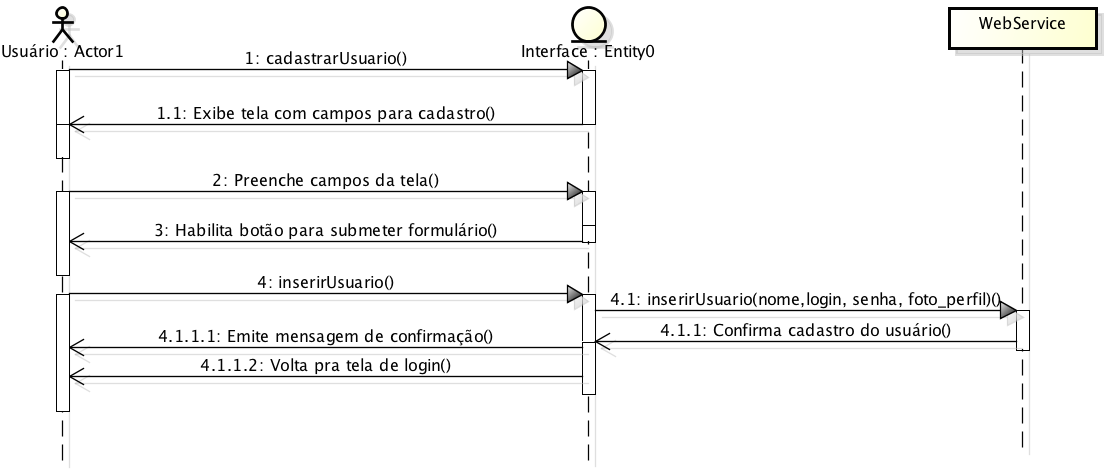
\includegraphics[width=17cm]{images/Diagramas/Diagram_de_Sequencia-Cadastrar_Usuario.png}
  \caption{Diagrama de Sequ\^{e}ncia 01 - Cadastrar Usu\'{a}rio}
  \label{fig:diagramaSequenciaCadastroUsuario}
\end{center}
\end{figure}

\subsection{Diagrama de Sequência 02 - Inserir Ocorrência}
\begin{figure}[!h]
\begin{center}
  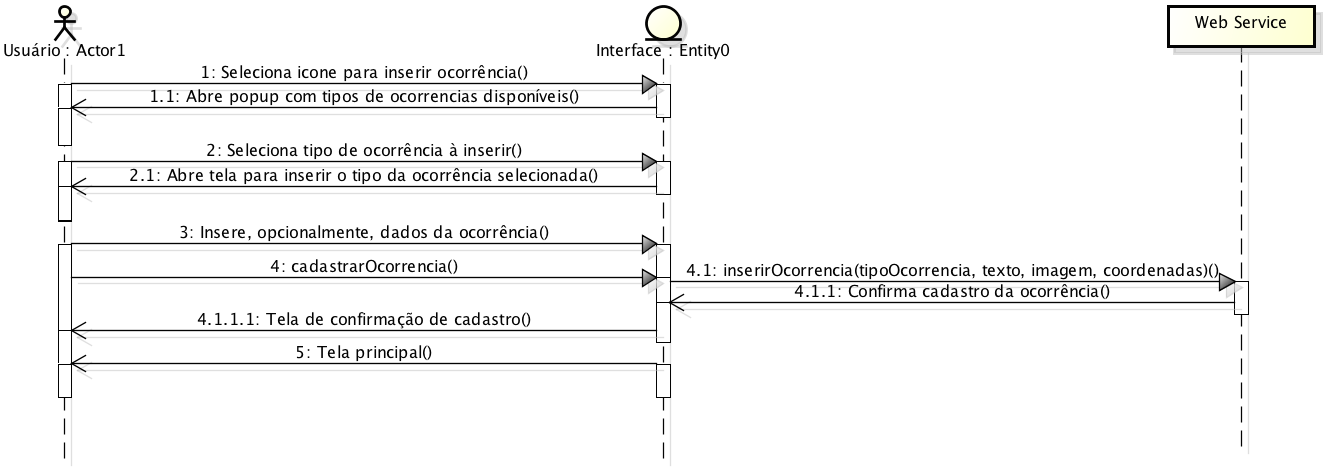
\includegraphics[width=7cm]{images/Diagramas/Diagram_de_Sequencia-Inserir_Ocorrencia.png}
  \caption{Diagrama de Sequ\^{e}ncia 02 - Inserir Ocorr\^{e}ncia}
  \label{fig:diagramaSequenciaInserirOcorrencia}
\end{center}
\end{figure}

\subsection{Diagrama de Sequência 03 - Buscar Destino}
\begin{figure}[!h]
\begin{center}
  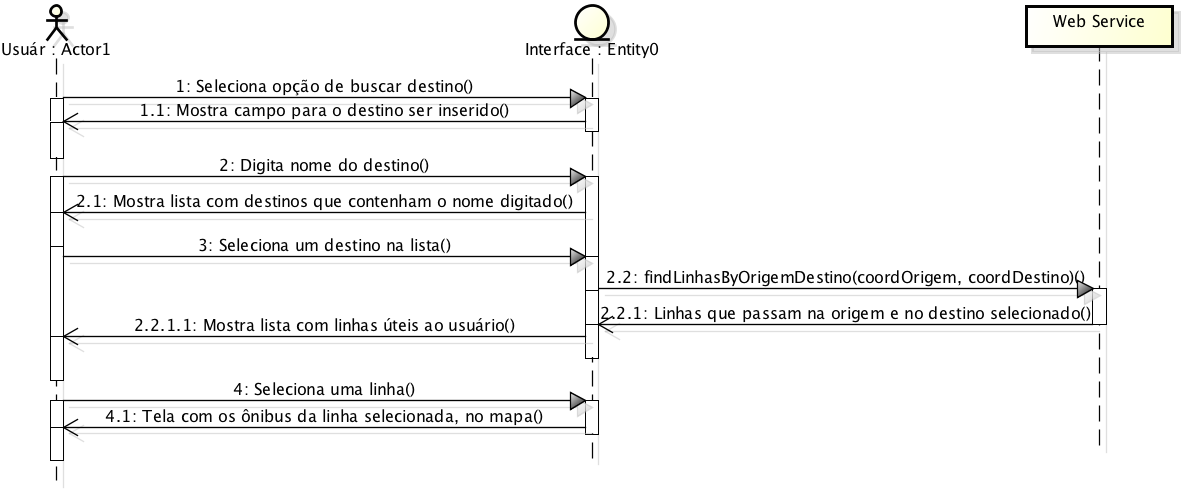
\includegraphics[width=7cm]{images/Diagramas/Diagram_de_Sequencia-Buscar_Destino.png}
  \caption{Diagrama de Sequ\^{e}ncia 03 - Buscar Destino}
  \label{fig:diagramaSequenciaBuscarDestino}
\end{center}
\end{figure}

\subsection{Diagrama de Sequência 04 - Buscar Ônibus}
\begin{figure}[!h]
\begin{center}
  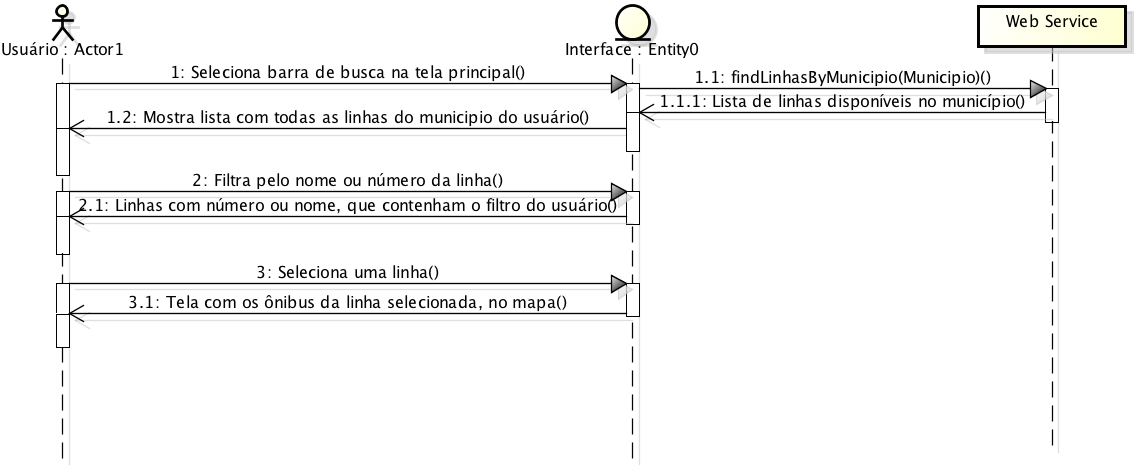
\includegraphics[width=7cm]{images/Diagramas/Diagram_de_Sequencia-Buscar_Onibus.png}
  \caption{Diagrama de Sequ\^{e}ncia 04 - Buscar \^{O}nibus}
  \label{fig:diagramaSequenciaBuscarOnibus}
\end{center}
\end{figure}

\subsection{Diagrama de Sequência 05 - Monitorar Ônibus}
\begin{figure}[!h]
\begin{center}
  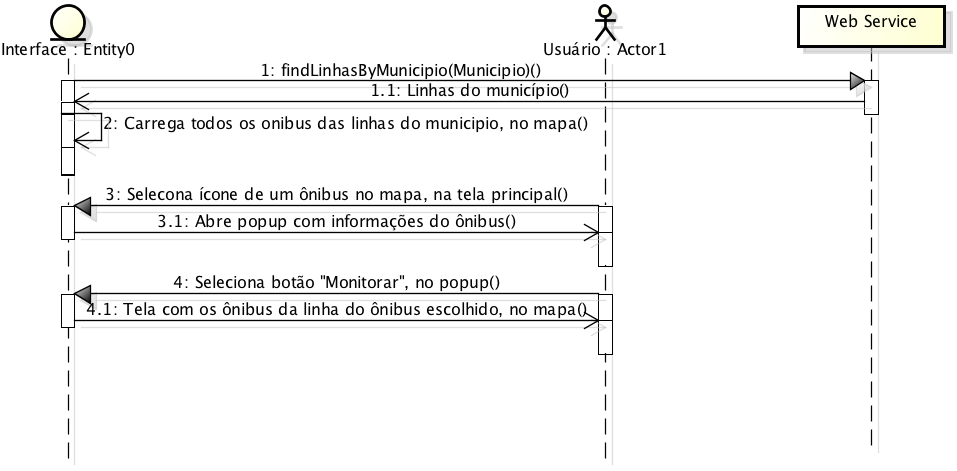
\includegraphics[width=7cm]{images/Diagramas/Diagram_de_Sequencia-Monitorar_Onibus.png}
  \caption{Diagrama de Sequ\^{e}ncia 05 - Monitorar \^{O}nibus}
  \label{fig:diagramaSequenciaMonitorarOnibus}
\end{center}
\end{figure}


\section{Telas e Funcionalidades}
\label{sc:telas}

\subsection{Cadastro de Usuário}

\begin{figure}[htp]
\begin{center}
  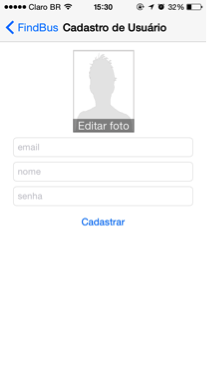
\includegraphics[width=5cm]{images/telas/cadastroDeUsuario.png}
  \caption{Tela de cadastro de usuário}
  \label{fig:telaCadastro}
\end{center}
\end{figure}

Para que se tenha acesso ao sistema é necessário que se faça um breve cadastro de usuário, onde é preciso informar, obrigatoriamente,  o email, nome e a senha do usuário que deseja ter acesso ao aplicativo. O usuário, caso deseje, pode informar, também, uma foto para compor seu perfil no sistema, conforme pode ser visto na \figref{fig:telaCadastro}.

O cadastro de usuário se fez necessário pela característica colaborativa do aplicativo, onde a maior parte das informações existentes são provenientes dos usuários. Exigindo, portanto, que se tenha um controle e, sobretudo, uma moderação de tudo que está sendo inserido por eles, garantido, assim, a qualidade e confiabilidade de todas as informações apresentadas.

\subsection{Login de Usuário – Autenticação}

O sistema fornece uma tela de autenticação de usuário, onde todo usuário, previamente cadastrado, pode ter acesso ao sistema. Para realizar o login no sistema, o usuário precisa, necessariamente, informar seu email e senha cadastrados, conforme ilustrado na \figref{fig:telaLogin}. Uma vez logado, o usuário consegue ter acesso a todas as informações existentes no aplicativo e só precisará passar novamente pelo processo de login caso opte por se desconectar do sistema, processo popularmente conhecido como logout. Isso acontece porque o sistema guarda o estado do usuário do sistema, o significar dizer que se o mesmo está logado não precisa passar pelo processo de autenticação novamente.

\begin{figure}[htp]
\begin{center}
  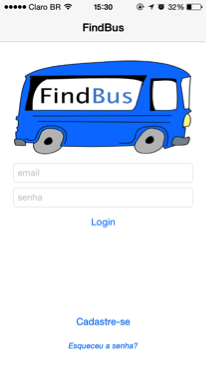
\includegraphics[width=5cm]{images/telas/loginDeUsuario.png}
  \caption{Tela de Login de usuário}
  \label{fig:telaLogin}
\end{center}
\end{figure}

Caso o usuário esqueça sua senha, esta mesma tela fornece a possibilidade de recuperação de senha, conforme pode ser visto na \figref{fig:telaLogin}. Para tanto, é necessário que o usuário informe seu email e, caso ele seja um usuário do sistema, receberá uma nova senha no email informado. Assim, ele pode ter acesso novamente ao sistema e, caso deseje, alterar sua senha. 

\subsection{Perto de você!}

Após efetuar login no sistema, o usuário é encaixado no contexto da cidade que ele se encontra. Isto é, o sistema consegue identificar a cidade que o usuário está e, dessa forma,  passa a mostrar tudo que está acontecendo no sistema de transporte público, bem como no trânsito dessa região. 
	
A tela para qual o usuário é direcionado após o login, ilustrada na figura \figref{fig:telaPrertoDeVoce}, é considerada a tela principal do sistema e consiste num mapa onde o usuário consegue visualizar todos os ônibus, incidentes de trânsito e pontos de ônibus que estão por perto. Assim, tendo uma visão geral do atual cenário dos serviços de transporte, bem como do trânsito da região que ele se encontra.  

\begin{figure}[htp]
\begin{center}
  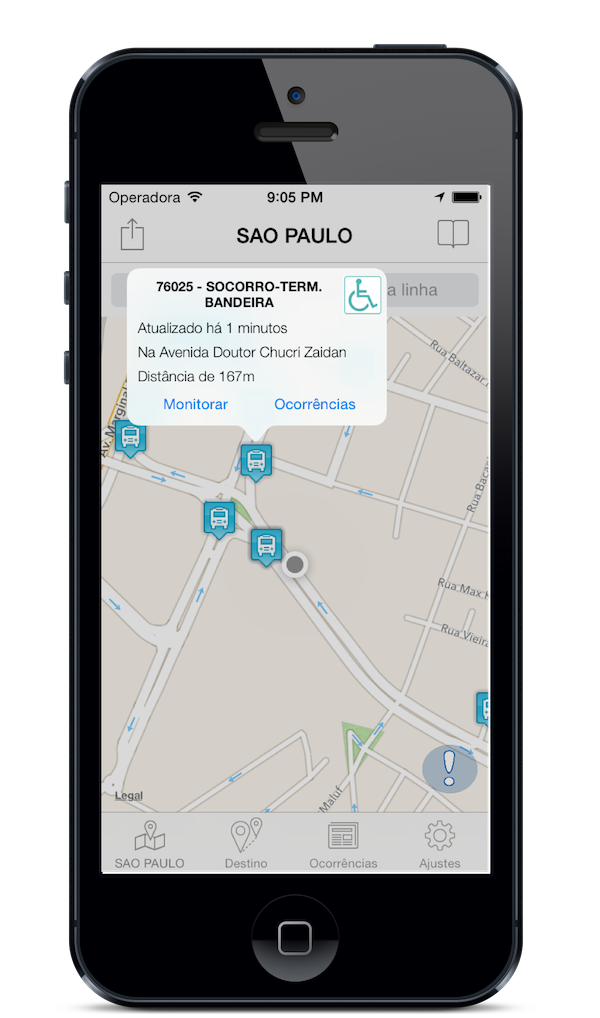
\includegraphics[width=6cm]{images/telas/pertoDeVoce.png}
  \caption{Tela principal do FindBus}
  \label{fig:telaPrertoDeVoce}
\end{center}
\end{figure}

	
Ademais, essa tela também permite que o usuário possa escolher uma linha específica para, assim, visualizar somente informações relacionadas a mesma, como por exemplo, os ônibus que estão rodando para linha escolhida, as ocorrências que estão afetando os ônibus dessa linha e os pontos de ônibus nos quais os passageiros dessa linha podem ter acesso aos veículos. Para tanto, o sistema mostra todas as linhas existentes na cidade que o usuário se encontra, a quantidade de ônibus que está rodando para cada linha no momento, bem como permite que o usuário possa encontrar uma linha pelo nome ou código da mesma, conforme pode ser visualizado na segunda tela apresentada na \figref{fig:telaPrincipal}.
	
Ainda na tela principal do sistema, ao clicar em um ícone no mapa, que pode se tratar de um  ônibus, ponto de ônibus ou ocorrências, o usuário consegue ter informações do tipo: endereço da localização do ícone escolhido; nome e código da linha, em caso de ônibus; distância do ícone clicado para o usuário; saber se um ônibus possui acessibilidade; quando foi a ultima atualização da localização do ônibus no sistema.
	
Nesse sentido, na tela em questão, o usuário consegue ter visão geral e um acesso rápido as principais funcionalidades do sistema. Como por exemple, monitoramento de uma linha, que é apresentado na próxima subseção.

\subsection{Monitoramento}

O sistema permite que o usuário escolha uma linha para ser monitorada. Para tanto, na tela principal, apresentada na subseção anterior, o usuário pode escolher um ônibus qualquer do mapa para passar a monitorar tanto ele quanto a linha que ele está fazendo no momento. Após a escolha, o usuário é direcionado para tela de monitoramento, ilustrada na figura \figref{fig:telaMonitoramento}, onde o mesmo poderá acompanhar em, praticamente, tempo real o deslocamento do seu ônibus, bem como tudo pode evidenciar um motivo de um possível atraso.
	
Conforme pode ser observado na \figref{fig:telaMonitoramento}, a tela de monitoramento mostra ao usuário o ônibus que o mesmo escolheu para monitorar, destacando-o com a cor branca, mas também permite que o usuário veja todos os demais ônibus da linha, pois todos eles fazem o mesmo trajeto do veículo escolhido e, portanto, também podem servir para ele. Ainda na tela de monitoramento, o usuário consegue visualizar o deslocamento de todos os ônibus em, praticamente, tempo real, visualizar  todas os incidentes de trânsitos, cadastrados por usuários que estão vivenciando o problema, que estão afetando a linha monitorada no memento, todas as paradas de ônibus da linha e informações de distância de um ônibus para um ponto, uma ocorrência ou para o próprio o usuário. Ademais,  nessa tela é possível visualizar todo trajeto feito pelos ônibus da linha monitorada, fazendo, assim, com que o usuário saiba todo itinerário, tanto de ida quanto de volta, de todos os ônibus e linhas da cidade. 
	
\begin{figure}[htp]
\begin{center}
  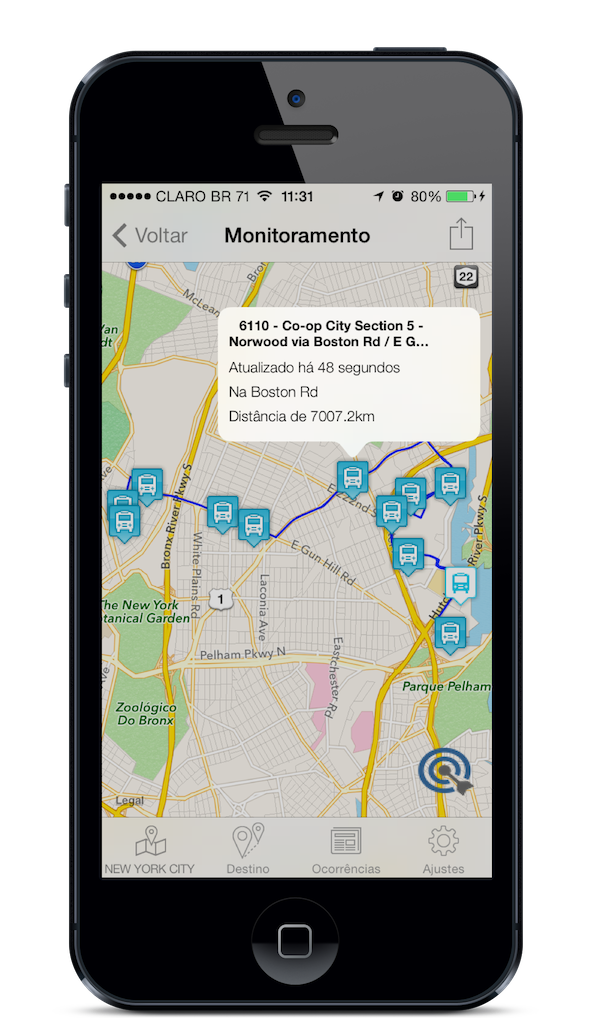
\includegraphics[width=5cm]{images/telas/monitoramento1.png}
  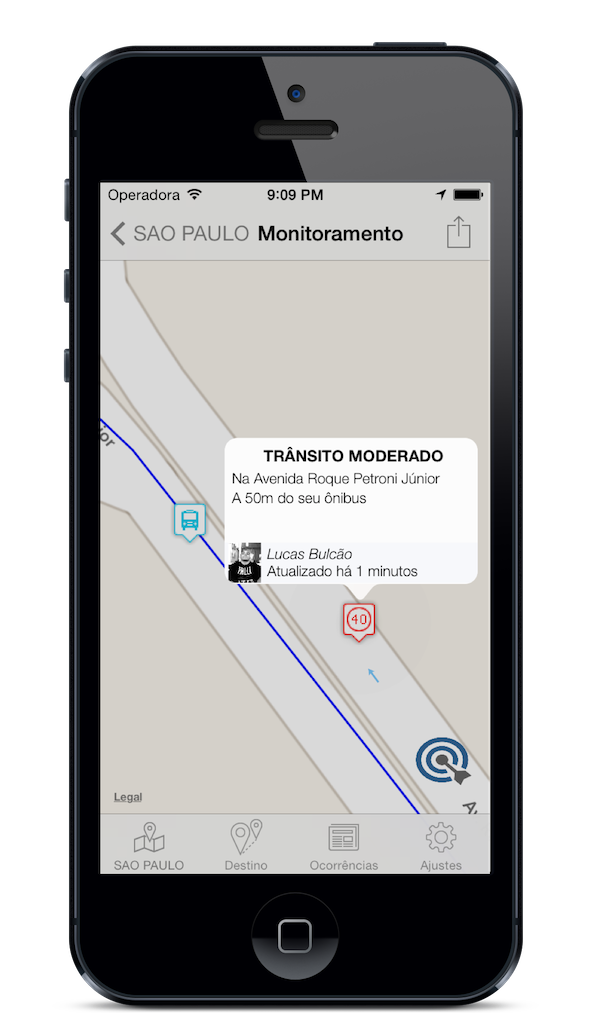
\includegraphics[width=5cm]{images/telas/monitoramento2.png}
  \caption{Tela de Monitoramento}
  \label{fig:telaMonitoramento}
\end{center}
\end{figure}

Isto posto, essa tela tem o objetivo de aumentar o poder de decisão do usuário, permitindo que o mesmo possa saber em tempo real todos os serviços disponíveis, bem como tudo que está acontecendo com uma determinada linha ou ônibus da cidade que ele se encontra.

\subsection{Cadastro de Ocorrências}

Na tela apresentada na \figref{fig:telaCadastroDeOcorrencia}, de maneira simples e intuitiva, o usuário consegue colaborar com outros usuários do sistema inserindo diversos tipos de ocorrências: ocorrência referente a atual situação do trânsito, que pode está moderado, intenso ou, literalmente, parado; a existência de uma barreira em um determinado ponto da cidade; que indique um local que está tendo obra; que a polícia está fazendo uma operação em determinado ponto da cidade; que ocorreu um acidente em um local da cidade, podendo informar se o mesmo foi um acidente leve ou grave; algum outro tipo de incidente que o usuário queira informar.
	
Para inserir a ocorrência, o usuário pode optar por anexar uma foto do fato, bem como detalhar a ocorrência digitando um texto, conforme pode ser visualizado na \figref{fig:telaCadastroDeOcorrencia}. Não obstante, para enviar uma ocorrência, é necessário que o usuário esteja, no mínimo, a 300 metros de uma rota de ônibus, ou seja, o sistema valida se o usuário realmente está em um local que seja rota de um veículo do transporte público da cidade. Desta forma, é possível associar cada ocorrência a diversas rotas e, por conseguinte, saber quais linhas de ônibus estão sendo afetadas por um determinada ocorrência.
	
\begin{figure}[htp]
\begin{center}
  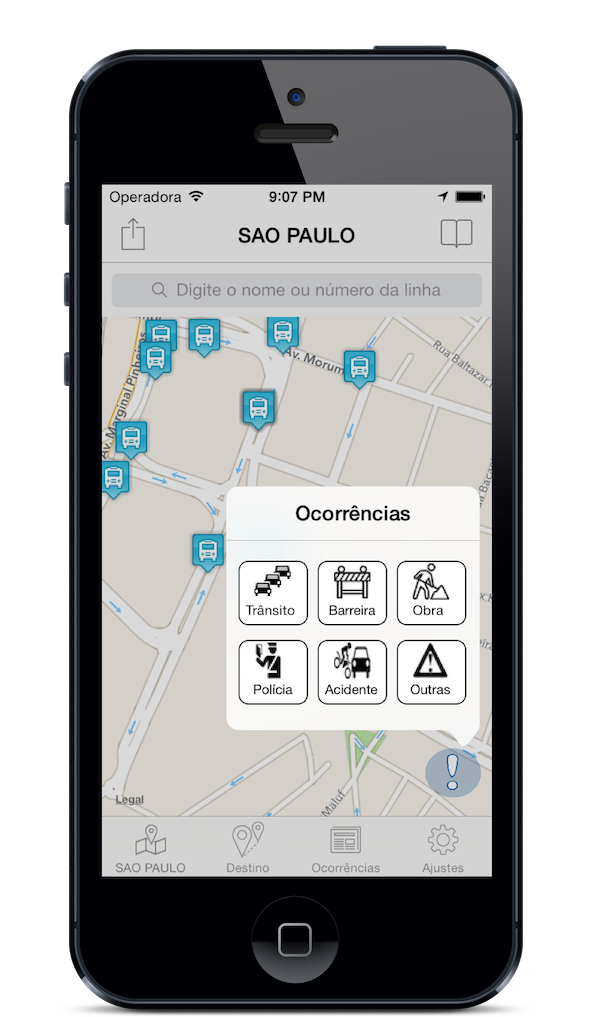
\includegraphics[width=5cm]{images/telas/cadastroDeOcorrencia.png}
   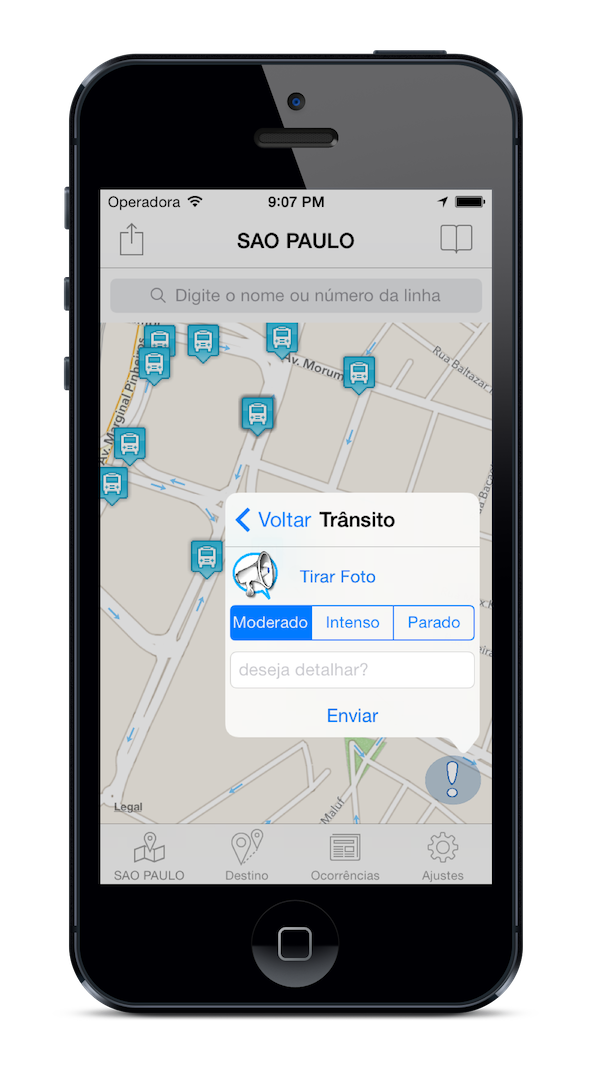
\includegraphics[width=5cm]{images/telas/cadastroDeOcorrencia2.png}
  \caption{Tela de Cadastro de Ocorrência}
  \label{fig:telaCadastroDeOcorrencia}
\end{center}
\end{figure}

Portanto, essa tela propicia um ambiente colaborativo, onde as pessoas podem rapidamente informar os problemas que estão vivenciado na cidade para que outras pessoas fiquem cientes do cenário atual e, desta forma, possa tomar a melhor decisão de como se deslocar dentro da cidade. 

\subsection{Visualização de ocorrências }

Um sistema possui uma tela, ilustrada na \figref{fig:telaVisualizarOcorrencia}, onde é possível visualizar todas as ocorrências que estão sendo inseridas no contexto que o usuário se encontra. Isto é, quando o usuário entra na listagem de ocorrência consegue visualizar, apenas, as ocorrências da sua cidade, tendo essas ocorrências organizadas de acordo com a distância para com o usuário e pelo quanto essas ocorrências afetam as linhas escolhidas como favoritas pelo mesmo.   
	
Ao clicar em uma ocorrência da listagem, o usuário consegue visualizar todos os detalhes da mesma: o nome do usuário que cadastrou a ocorrência; quanto tempo faz que a ocorrência foi inserida; o tipo da ocorrência; o endereço de onde aconteceu o fato; a foto anexada a ocorrência; todas as linhas que estão sendo afetada de algum modo pela ocorrência no momento.  
	
A ideia dessa tela é fazer com o usuário tenha um acesso rápido a tudo que está acontecendo no tocante ao trânsito e aos serviços de transporte público da cidade por aqueles que estão vivenciando o problema. 

\begin{figure}[htp]
\begin{center}
  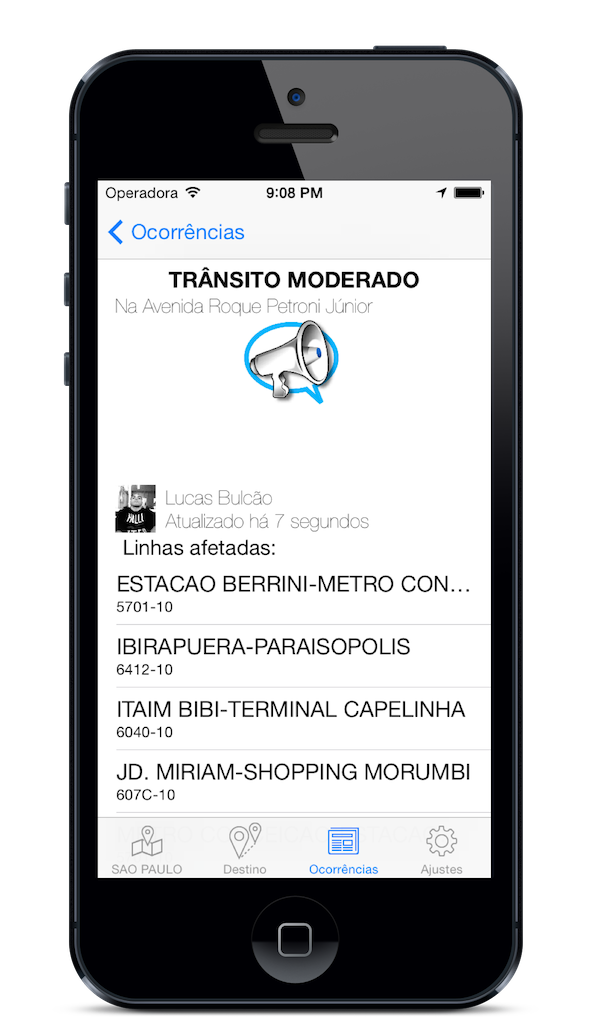
\includegraphics[width=6cm]{images/telas/visualizarOcorrencia.png}
  \caption{Tela de Visualização de Ocorrência}
  \label{fig:telaVisualizarOcorrencia}
\end{center}
\end{figure}

\subsection{Como chegar?}

A \figref{fig:telaRecomendacao} apresenta a tela de recomendação de linha, que consiste em mostrar ao usuário como ele pode chegar a um determinado destino a partir do local que ele se encontra. Para tanto, o usuário informa, de maneira simples e intuitiva, o nome ou endereço do seu destino e o sistema verifica quais linhas passam pelos pontos de ônibus mais próximos dele e que também passam nos pontos mais próximos do destino escolhido. 
	
Para recomendar a melhor linha ao usuário, o sistema utiliza como parâmetro a distância do usuário para seu destino utilizando cada linha, bem como a situação atual do trânsito no itinerário de cada linha que poderá levá-lo a seu destino. Ou seja, além da distância, o sistema se  utiliza das ocorrências inseridas pelos colaboradores para poder recomendar a melhor linha de ônibus para o usuário chegar no seu destino. Dessa forma, as linhas mais recomendadas sempre estarão mais ao topo da listagem, sendo que uma linha com uma distância maior que outra pode estar mais ao topo quando a mesma não possuir nenhuma ocorrência afetando-a e a outra possuir uma ocorrência de trânsito parado e acidente, por exemplo.
	
\begin{figure}[htp]
\begin{center}
  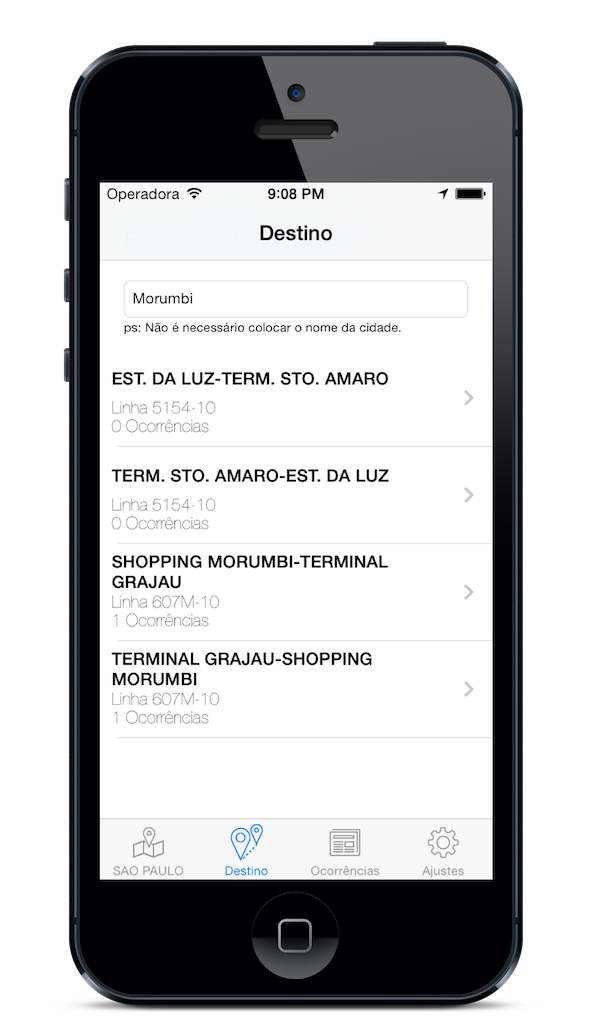
\includegraphics[width=6cm]{images/telas/comoChegar.png}
  \caption{Tela de Recomendação de Linha}
  \label{fig:telaRecomendacao}
\end{center}
\end{figure}

Nesse sentido, o sistema consegue recomendar a melhor linha para o usuário se deslocar de um determinado ponto a outro da cidade no menor tempo possível.

\subsection{Linhas Favoritas}

Conforme mostrado na \figref{fig:telaFavoritas}, o aplicativo permite que o usuário possa escolher linhas, dentre as existentes no serviço legal de transporte público, como favoritas para cada cidade que o sistema opera. Isto é, o usuário pode ter linhas favoritas para cidade de São Paulo e linhas favoritas na cidade de New York, por exemplo. Desta forma, ao entrar no sistema o usuário pode ter um acesso rápido, a partir da tela principal, às linhas que foram favoritadas no contexto que ele se encontra.
	
Como uma cidade, normalmente, possui uma grande quantidade de linhas, a tarefa de procurar por uma linha específica pode se tornar entediante, uma vez que pode ser uma linha que comumente o usuário necessita buscar. Portanto, permitir que os usuários possam escolher as linhas que costumeiramente por eles são utilizadas, para que se tenha um acesso rápido toda vez que necessário for é algo, indiscutivelmente, válido e, sobretudo, essencial.
	
\begin{figure}[htp]
\begin{center}
  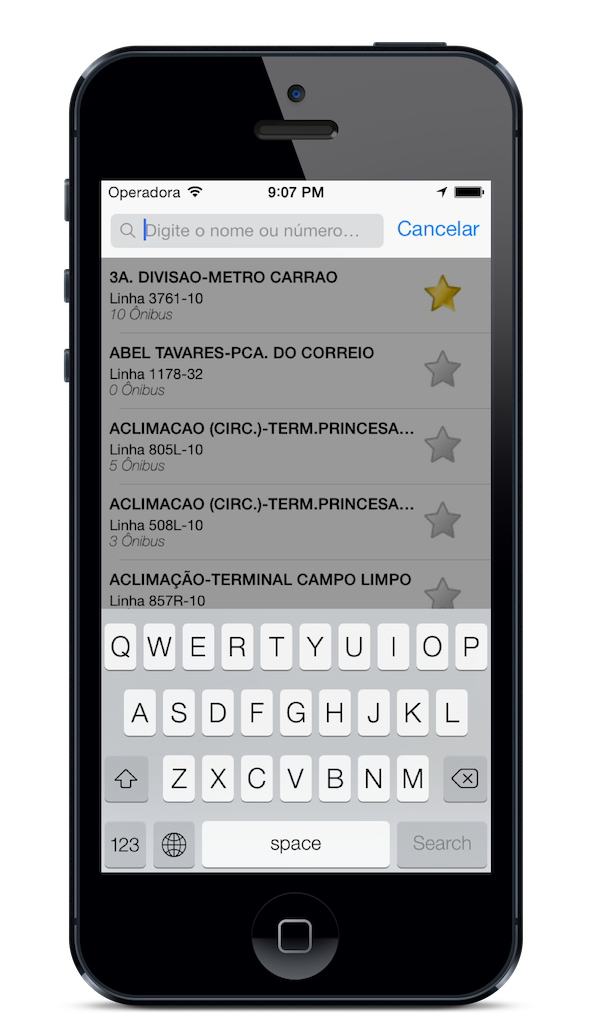
\includegraphics[width=6cm]{images/telas/linhasFavoritas.png}
  \caption{Tela de Linhas Favoritas}
  \label{fig:telaFavoritas}
\end{center}
\end{figure}


Quando um usuário escolhe determinada linha como favorita, o mesmo passa a receber algumas notificações em background sobre a proximidade dos ônibus que operam para essa linha. Tal funcionalidade é apresentada em detalhes na subseção subsequente. 

\subsection{Notificações em Background}

Conforme mencionado na seção anterior, no momento que o usuário escolhe uma linha como favorita, além de poder ter um acesso rápido a essa, o mesmo passa a receber notificações, em background, contendo informações sobre a proximidade de todos os ônibus que estão operando para linha escolhida. O alerta é transmitido para o usuário no exato momento que algum ônibus que está rodando para uma das linhas favoritadas entra no raio de 1 quilometro do usuário. 

Conforme pode ser visualizado na \figref{fig:telaNotificacao}, a notificação mostra a identificação do ônibus, também conhecido como prefixo, para qual linha favorita este ônibus opera, o endereço em que o veículo se encontra, a distância do ônibus para o usuário, bem como em quanto tempo este ônibus vai chegar. Depois que o ônibus entra em um raio de 1 quilometro do usuário, o sistema tem até 20 segundos para  enviar um alerta para o usuário.
	
O usuário pode escolher, também, para quais linhas favoritadas ele deseja ficar recebendo as notificações. Para tanto, basta entrar na tela das linhas favoritas, apresentada na \figref{fig:telaNotificacao}, e optar por receber ou não as notificações para determinada linha.

\begin{figure}[htp]
\begin{center}
  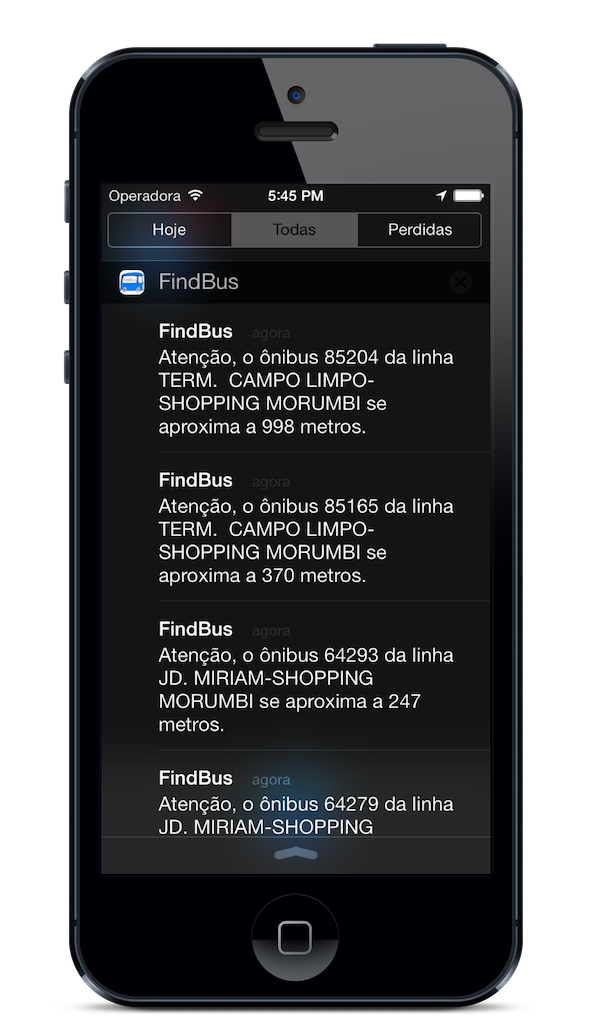
\includegraphics[width=6cm]{images/telas/notificacao.png}
  \caption{Tela de Notificação de Proximidade}
  \label{fig:telaNotificacao}
\end{center}
\end{figure}

\subsection{Paradas de ônibus}

São tantas paradas de ônibus existentes em uma cidade que é, praticamente, impossível saber a localização de todas elas. Além disso, saber quais linhas passam por cada parada dessa é algo ainda mais improvável. Para solucionar esse problema, o sistema permite que o usuário possa visualizar, a partir de qualquer mapa apresentado no aplicativo, todas as paradas de ônibus existentes na cidade que ele se encontra.
	 
Ao clicar em qualquer ponto de ônibus mostrado no mapa, o usuário consegue saber informações a respeito da localização exata da parada, sua distância para o ponto escolhido e, caso esteja na tela de monitoramento, para o ônibus monitorado, bem como quais linhas passam por esse ponto.

\begin{figure}[htp]
\begin{center}
  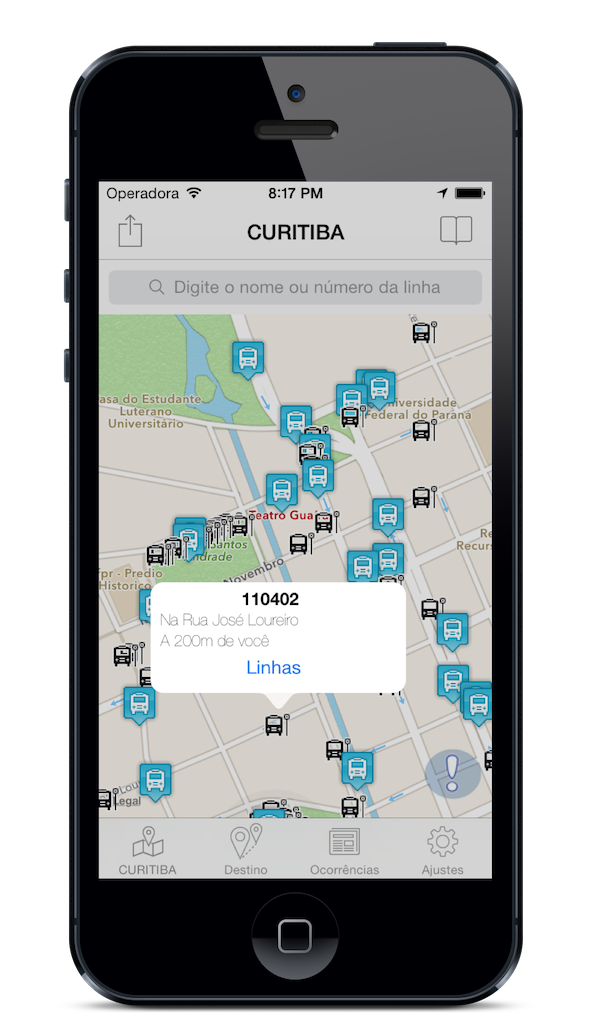
\includegraphics[width=6cm]{images/telas/paradas.png}
  \caption{Paradas de ônibus}
  \label{fig:telaParadas}
\end{center}
\end{figure}


\chapter{Avaliação e Validação}
\label{ch:avaliacao}

\section{Prova de Conceito – Avaliação da Proposta}
\label{sc:provaConceito}

Com a finalidade de verificar se os objetivos que fora especificados neste trabalho, realmente, foram atingidos com o desenvolvimento do aplicativo apresentado, foi realizado uma prova de conceito. O intuito da prova de conceito é criar um modelo prático que possa provar o conceito estabelecido por uma pesquisa ou artigo técnico, isto é, não se faz necessário que o experimento esteja totalmente finalizado, mas que permita demonstrar como o mesmo pode contribuir para a colaboração, bem como a produção de conhecimento [TONELLA].

A prova de conceito foi realizada no período de 11 a 13 de novembro de 2014 e consistiu na elaboração de um questionário de avaliação da versão 1.0.5  do aplicativo FindBus, lançada em março de 2014 e disponível na App Store, loja de aplicativo da Apple, bem como da versão 1.0.1 lançado em setembro de 2015 na Google Play, loja de aplicativo da Google. O questionário está disponível, bem como pode ser visualizado no Apêndice A deste trabalho.

O questionário de avaliação conteve 25 questões e foi dividido em duas etapas: etapa de reconhecimento e etapa de avaliação. A primeira teve como objetivo reconhecer o perfil do usuário, bem como verificar se o mesmo estaria apto a avaliar o aplicativo. A segunda etapa consistiu em 22 perguntas diretamente relacionadas ao uso da aplicação, objetivando, assim, realmente avaliar se a proposta está funcionando conforme fora especificada. 

O questionário de avaliação foi enviado para o e-mail de 3000 usuários, todos eles com mais de 3 meses de uso. Nesse ínterim, foi possível coletar 63 respostas para o questionário e, como base nelas, os resultados da realização da prova de conceito foram expressos na seção subsequente. 

\section{Apresentação dos resultados}
\label{sc:apresentacaoResultados}

O questionário foi desenvolvido com base nos objetivos descritos na seção \ref{sc:objetivo} deste trabalho, onde o principal objetivo foi, exatamente, certificar-se de que a proposta desenvolvida atendia todos os objetivos apresentados. Para tanto, conforme mencionado no início desta seção, criou-se um questionário utilizando o Google Forms, ferramenta da Google para criação de formulários, contendo 25 questões. A referida pesquisa ficou disponível por um período de três dias e foi possível obter, nesse ínterim, 63 respostas para a mesma.  

A ideia da pesquisa de avaliação não foi analisar os dados fornecidos de forma individual, mas sim segmentá-los apenas para análise estatística. A participação foi voluntária e, como nenhum participante precisou se identificar, os dados foram anônimos e confidenciais.    

Doravante os dados das principais perguntas serão apresentados obedecendo a seguinte estrutura: questão; apresentação dos dados em uma tabela e, quando necessário, apresentação dos dados em um gráfico; breve comentário sobre os resultados, isto é, uma análise parcial dos dados.

\textbf{Questão 1:  Qual plataforma você está utilizando?}

\begin{center}
\begin{longtable}{c|c|c}
\hline
    \multicolumn{1}{c}{\textbf{Resultado}} & \multicolumn{1}{c}{\textbf{Quantidade}} & \multicolumn{1}{c}{\textbf{Percentual}} \\
\hline
    IOS & 47 &  75\%\\
    \hline
    Android & 16 & 25\%\\
    \hline
\caption{Tabela de resultados obtidos na questão 1}
\end{longtable}
\end{center}


\begin{figure}[h]
\begin{center}
  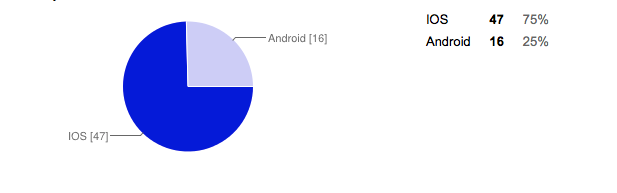
\includegraphics[width=12cm]{images/graficos/questao1.png}
  \caption{Gráfico de resultados da questão 1}
  \label{fig:questao1}
\end{center}
\end{figure}

\textbf{Comentários:}

O objetivo dessa pergunta foi avaliar se os objetivos descritos neste trabalho foram atendidos para todas as plataformas para quais a proposta foi desenvolvida. Não obstante, como as respostas foram bastante similares para ambas plataformas, os dados não foram analisados separadamente. 

Observa-se que 75\% dos usuários que participaram da pesquisa utilizam a ferramenta desenvolvida para plataforma IOS, enquanto que 25\% utilizam a plataforma Android.\newline

\textbf{Questão 2: Ao logar no aplicativo, o sistema conseguiu identificar a cidade onde você se encontra?}

\begin{center}
\begin{longtable}{c|c|c}
\hline
    \multicolumn{1}{c}{\textbf{Resultado}} & \multicolumn{1}{c}{\textbf{Quantidade}} & \multicolumn{1}{c}{\textbf{Percentual}} \\
\hline
    Sim & 61 &  97\%\\
    \hline
    Não & 2 & 3\%\\
    \hline
\caption{Tabela de resultados obtidos na questão 2}
\end{longtable}
\end{center}


\begin{figure}[h]
\begin{center}
  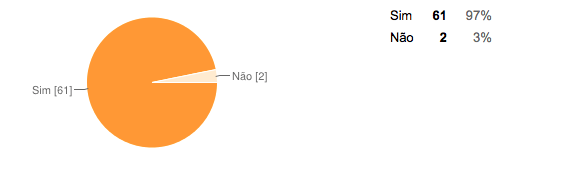
\includegraphics[width=16cm]{images/graficos/questao2.png}
  \caption{Gráfico de resultados da questão 2}
  \label{fig:questao1}
\end{center}
\end{figure}

\textbf{Comentários:}

O objetivo dessa pergunta foi avaliar a sensibilidade ao contexto existente na aplicação, pois se a mesma consegue identificar a cidade, ou seja, o contexto de localização que o usuário se encontra, ela consegue encaixar o usuário no contexto correto, em outras palavras, dessa forma, é possível mostrar para os usuários todos os ônibus, linhas, pontos, incidentes, bem como todas as informações no tocante a sua cidade.
	
Observa-se, através do gráfico mostrado na figura \figref{fig:questao1}, que 97\% dos usuários afirmaram que realmente o sistema consegue identificar em qual cidade o usuário se encontra, enquanto que, apenas, 3\% afirmaram o contrário. \newline

\textbf{Questão 3:  Você se encontra em uma cidade atendida pelo aplicativo (São Paulo, Curitiba, New York e Boston)?}

\begin{center}
\begin{longtable}{c|c|c}
\hline
    \multicolumn{1}{c}{\textbf{Resultado}} & \multicolumn{1}{c}{\textbf{Quantidade}} & \multicolumn{1}{c}{\textbf{Percentual}} \\
\hline
    Sim & 44 &  70\%\\
    \hline
    Não & 19 & 30\%\\
    \hline
\caption{Tabela de resultados obtidos na questão 3}
\end{longtable}
\end{center}


\begin{figure}[h]
\begin{center}
  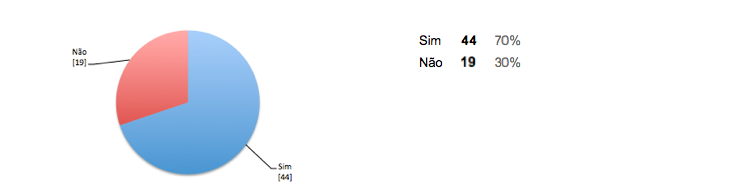
\includegraphics[width=16cm]{images/graficos/questao3.png}
  \caption{Gráfico de resultados da questão 3}
  \label{fig:questao3}
\end{center}
\end{figure}

\textbf{Comentários:}

Atualmente, o aplicativo está funcionando nas cidades de São Paulo, Curitiba, Boston e New York. Portanto, somente os usuários que utilizam o aplicativo em umas dessas cidades possuem condições de avaliar todas as funcionalidades contidas no mesmo. Isto posto, o principal objetivo da pergunta foi exatamente identificar as pessoas que  poderiam prosseguir para segunda etapa do questionário, a etapa de avaliação. 
	
Observa-se que 44 pessoas, do universo de 63 usuários, que responderam o questionário estavam em uma das cidades atendidas pelo aplicativo, o que representa um total de 70\% do total de entrevistados. Nota-se que, como a pergunta determinava o fim ou o prosseguimento do questionário, apenas 44 pessoas deram continuidade e passaram para etapa de avaliação, o que significa dizer o que a partir da próxima pergunta o número de respostas passará de 63 para 44, sendo assim, tivemos na etapa de avaliação 70\% das pessoas que se propuseram a responder o questionário.\newline

\textbf{Questão 4: Ao logar, você é direcionado para tela principal do sistema. Nessa tela, você consegue visualizar os ônibus que estão perto de sua localização?}

\begin{center}
\begin{longtable}{c|c|c}
\hline
    \multicolumn{1}{c}{\textbf{Resultado}} & \multicolumn{1}{c}{\textbf{Quantidade}} & \multicolumn{1}{c}{\textbf{Percentual}} \\
\hline
    Sim & 40 &  63\%\\
    \hline
    Não & 04 & 6\%\\
    \hline
\caption{Tabela de resultados obtidos na questão 4}
\label{tabq4}
\end{longtable}
\end{center}


\begin{figure}[h]
\begin{center}
  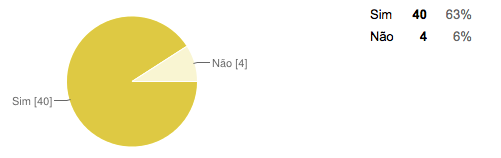
\includegraphics[width=16cm]{images/graficos/questao4.png}
  \caption{Gráfico de resultados da questão 4}
  \label{fig:questao4}
\end{center}
\end{figure}

\textbf{Comentários:}

Algumas das perguntas criadas no questionário de avaliação tiveram o objetivo de guiar o usuário, apresentar a aplicação, bem como garantir que o usuário realmente utilizou o aplicativo. Deste modo, fazendo com que os dados colhidos, sobretudo nas questões cuja finalidade é validar os objetivos propostos neste trabalho, sejam fidedignos. Não obstante, os dados coletados nessa questão comprovam, conforme pode ser visto no gráfico da figura  \figref{fig:questao4} e na tabela \ref{tabq4}, o quão o aplicativo se preocupa com a localização do usuário, em mostrar o que está acontecendo ao seu redor.\newline

\textbf{Questão 5: Ao clicar em um determinado ônibus, o nível de informação mostrada pelo aplicativo é suficiente (linha, identificação do ônibus, tempo de atualização, distância, endereço)?}

\begin{center}
\begin{longtable}{c|p{1cm}|p{1cm}|p{2cm}|p{1cm}|p{1cm}}
\hline
    \multicolumn{1}{c}{\textbf{Item/Opção}} & \multicolumn{1}{c}{\textbf{Discordo Totalmente}} & \multicolumn{1}{c}{\textbf{Discordo}} & \multicolumn{1}{c}{\textbf{Nem discordo,nem concordo}} & \multicolumn{1}{c}{\textbf{Concordo}} & \multicolumn{1}{c}{\textbf{Concordo Totalmente}} \\
\hline
    Identificação da linha & 1 & 0 & 1 & 26 & 16\\
    \hline
    Identificação do ônibus & 1 & 0 & 2 & 26 & 15\\
    \hline
     Tempo de atualização & 1 & 0 & 11 & 20 & 6\\
    \hline
    Distância & 2 & 5 & 5 & 27 & 5\\
    \hline
     Endereço & 1 & 0 & 2 & 28 & 13\\
     \hline
\caption{Tabela de resultados obtidos na questão 4}
\label{tabq5}
\end{longtable}
\end{center}


\textbf{Comentários:}

O aplicativo se propõe a munir o usuário com o máximo de informação no tocante ao meio de transporte público que o mesmo comumente utilize, aumentando, dessa forma, o poder de decisão deste. Isto posto, com a finalidade de medir a qualidade, bem como a satisfação do usuário para com o nível de informação disponibilizada pelo aplicativo, a pergunta 5 teve como objetivo validar se as informações mostradas referentes a identificação da linha, identificação do ônibus, tempo de atualização do veículo, distância do veículo para o usuário e endereço onde o ônibus se encontra são realmente suficientes.
	
Analisando os dados disponíveis na tabela \ref{tabq5}, observa-se, de modo geral, que a maioria das pessoas que se propuseram a responder o questionário concordaram que o nível de informação mostrada no que tange aos ônibus é satisfatória. Contudo, vale ressaltar que quando se refere ao tempo de atualização o nível de satisfação não é tão bom como acontece com os outros itens avaliados na questão.\newline

\textbf{Questão 6: Na tela principal, ao tentar digitar o nome ou número de uma linha, você consegue encontrar todas as linhas existentes em sua cidade.}

\begin{center}
\begin{longtable}{c|c|c}
\hline
    \multicolumn{1}{c}{\textbf{Resultado}} & \multicolumn{1}{c}{\textbf{Quantidade}} & \multicolumn{1}{c}{\textbf{Percentual}} \\
\hline
    Concordo totalmente & 28 &  44\%\\
    \hline
    Concordo parcialmente & 14 & 22\%\\
    \hline
     Não concordo & 2 & 3\%\\
    \hline
\caption{Tabela de resultados obtidos na questão 6}
\label{tabq6}
\end{longtable}
\end{center}


\begin{figure}[h]
\begin{center}
  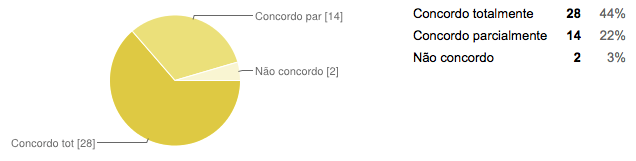
\includegraphics[width=16cm]{images/graficos/questao6.png}
  \caption{Gráfico de resultados da questão 6}
  \label{fig:questao6}
\end{center}
\end{figure}

\textbf{Comentários:}

Uma dos requisitos do aplicativo é exatamente fazer com que o usuário saiba todas as linhas existente na cidade que ele se encontra. Isto posto, a questão 6 foi criada com a finalidade de validar se realmente a aplicação atende tal requisito. 
	
Observa-se que 42 pessoas, do total de 44, concordam que o aplicativo consegue mostrar todas as linhas existente na cidade do usuário, enquanto que, apenas, 2 pessoas afirmaram o contrário. Nesse sentido, de maneira geral, analisando os dados apresentados no gráfico presente na figura \figref{fig:questao6}, nota-se que o aplicativo consegue, na maioria das vezes, mostrar aos seus usuários todas as linhas existentes na cidades em que estes se encontram.\newline

\textbf{Questão 7: Na aba de ocorrências, você consegue visualizar a ocorrência cadastrada, bem como quais linhas estão sendo afetadas pelo incidente informado?}

\begin{center}
\begin{longtable}{c|c|c}
\hline
    \multicolumn{1}{c}{\textbf{Resultado}} & \multicolumn{1}{c}{\textbf{Quantidade}} & \multicolumn{1}{c}{\textbf{Percentual}} \\
\hline
    Sim & 41 &  65\%\\
    \hline
    Não & 3 & 5\%\\
    \hline
\caption{Tabela de resultados obtidos na questão 7}
\label{tabq7}
\end{longtable}
\end{center}


\begin{figure}[h]
\begin{center}
  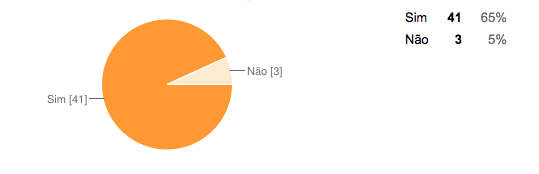
\includegraphics[width=16cm]{images/graficos/questao7.png}
  \caption{Gráfico de resultados da questão 7}
  \label{fig:questao7}
\end{center}
\end{figure}

\textbf{Comentários:}

A questão 7 tem como objetivo atestar se os usuários conseguem cadastrar ocorrências de incidentes de trânsito, sobretudo, se estes conseguem saber quais linhas estão sendo afetadas por tais eventos, exatamente como fora proposto nos objetivos deste trabalho.
	
Nota-se, analisando os dados apresentados, que a maioria das avaliações foram positivas, onde a maioria das pessoas conseguiram tanto cadastrar os incidentes vivenciados, como visualizar quais linhas o incidente estava afetando. \newline

\textbf{Questão 8: Na aba de destino, ao tentar encontrar as linhas que te levará até o destino informado, como você classifica a recomendação feita pelo aplicativo? }

\begin{center}
\begin{longtable}{c|c|c}
\hline
    \multicolumn{1}{c}{\textbf{Resultado}} & \multicolumn{1}{c}{\textbf{Quantidade}} & \multicolumn{1}{c}{\textbf{Percentual}} \\
\hline
    1 & 2 &  3\%\\
    \hline
    2 & 1 & 2\%\\
    \hline
    3 & 3 &  5\%\\
    \hline
    4 & 27 & 43\%\\
    \hline
    5 & 11 & 17\%\\
    \hline
\caption{Tabela de resultados obtidos na questão 8}
\label{tabq8}
\end{longtable}
\end{center}


\begin{figure}[h]
\begin{center}
  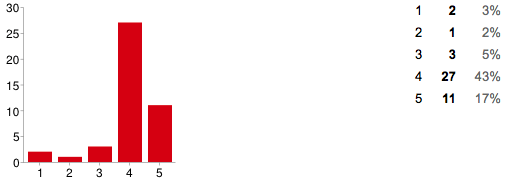
\includegraphics[width=16cm]{images/graficos/questao8.png}
  \caption{Gráfico de resultados da questão 8}
  \label{fig:questao8}
\end{center}
\end{figure}

\textbf{Comentários:}

Uma das funcionalidades que este trabalho propusera fornecer ao usuário é a recomendação de linhas, onde o mesmo conseguiria saber qual linha o levaria à um determinado destino a partir de um determinado ponto. Isto posto, a questão 8 tem o objetivo de validar se as linhas recomendadas pelo aplicativo realmente  servem para os usuários  chegarem até seus destinos. Para tanto, pediu-se aos participantes da avaliação que classificassem a recomendação feita pelo aplicativo com uma nota de 1 a 5, onde 1 representava uma total insatisfação e 5 uma total satisfação com a recomendação.

No gráfico mostrado na figura \figref{fig:questao8}, é possível observar uma concentração maior nas opções de classificação 4 e 5, o que comprova que a maioria dos participantes ficaram satisfeitos com a recomendação feita pelo aplicativo. Vale destacar que a satisfação não foi unanimidade, tendo, portanto, 3 avaliações, de um total  de 44, totalmente negativas. \newline

\textbf{Questão 9: Como você classifica o nível de informação disponibilizada pelo aplicativo?}

\begin{center}
\begin{longtable}{c|c|c}
\hline
    \multicolumn{1}{c}{\textbf{Resultado}} & \multicolumn{1}{c}{\textbf{Quantidade}} & \multicolumn{1}{c}{\textbf{Percentual}} \\
\hline
    1 & 3 &  5\%\\
    \hline
    2 & 1 & 2\%\\
    \hline
    3 & 2 &  3\%\\
    \hline
    4 & 29 & 46\%\\
    \hline
    5 & 9 & 9\%\\
    \hline
\caption{Tabela de resultados obtidos na questão 9}
\label{tabq9}
\end{longtable}
\end{center}


\begin{figure}[h]
\begin{center}
  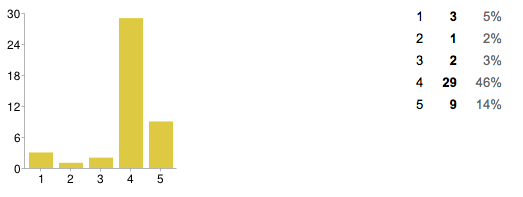
\includegraphics[width=16cm]{images/graficos/questao9.png}
  \caption{Gráfico de resultados da questão 9}
  \label{fig:questao9}
\end{center}
\end{figure}

\textbf{Comentários:}

O aplicativo se propõe a fornecer uma grande quantidade de informação à seus usuários, todavia, é necessário que se saiba o nível da informação disponibilizada. Para tanto, a questão 9 pediu para que os participantes da avaliação classificassem o nível de informação disponibilizada pelo aplicativo com uma nota no intervalo de 1 a 5, onde 1 significava dizer que o sistema fornecia um péssimo nível de informação, enquanto que 5 significava que o usuário considerava o nível de informação disponibilizada pelo aplicativo excelente. 
	
Análogo ao que aconteceu na questão 8, analisando o gráfico da figura \figref{fig:questao9}, observa-se uma concentração maior nas respostas 4 e 5, o que valida a satisfação da maioria dos usuários no que tange o nível de informação disponibilizada pela aplicação. \newline

\textbf{Questão 10: A utilização do FindBus ajuda a otimizar o tempo?}

\begin{center}
\begin{longtable}{c|c|c}
\hline
    \multicolumn{1}{c}{\textbf{Resultado}} & \multicolumn{1}{c}{\textbf{Quantidade}} & \multicolumn{1}{c}{\textbf{Percentual}} \\
\hline
    Ajuda totalmente & 23 &  37\%\\
    \hline
    Ajuda parcialmente & 19 & 30\%\\
    \hline
    Não ajuda & 2 &  3\%\\
    \hline

\caption{Tabela de resultados obtidos na questão 10}
\label{tabq10}
\end{longtable}
\end{center}


\begin{figure}[h]
\begin{center}
  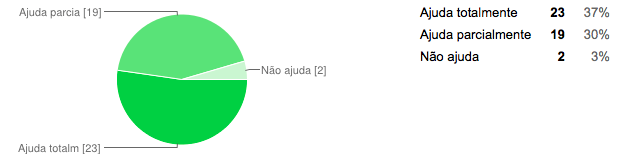
\includegraphics[width=16cm]{images/graficos/questao10.png}
  \caption{Gráfico de resultados da questão 10}
  \label{fig:questao10}
\end{center}
\end{figure}

\textbf{Comentários:}

Uma das grandes propostas do aplicativo proposto neste trabalho é fazer com que seus usuários possam otimizar o tempo ao utilizar os serviços de transporte público para se locomoverem. Portanto, a questão 10 foi criada com a finalidade de provar que o mesmo, realmente, consegue propiciar tal beneficio aos seus usuários. 
	
Analisando o gráfico ilustrado na figura \figref{fig:questao10}, nota-se que 42 pessoas, de um total de 44 avaliados, afirmaram que conseguem otimizar o tempo com a utilização do FindBus. Portanto, pode-se afirmar que com a utilização do aplicativo proposto neste trabalho é possível perder menos tempo ao se locomover pela cidade e, por conseguinte, aproveitar melhor o tempo disponível.\newline

\textbf{Questão 11: Como você classifica a localização e tempo de atualização da posição dos ônibus no aplicativo?}

\begin{center}
\begin{longtable}{c|c|c}
\hline
    \multicolumn{1}{c}{\textbf{Resultado}} & \multicolumn{1}{c}{\textbf{Quantidade}} & \multicolumn{1}{c}{\textbf{Percentual}} \\
\hline
    Muito ruim & 2 &  3\%\\
    \hline
    Ruim & 3 & 3\%\\
    \hline
    Aceitável & 12 &  19\%\\
    \hline
    Bom & 20 & 20\%\\
    \hline
    Muito bom & 7 & 7\%\\
    \hline
\caption{Tabela de resultados obtidos na questão 11}
\label{tabq11}
\end{longtable}
\end{center}

\begin{figure}[!h]
\begin{center}
  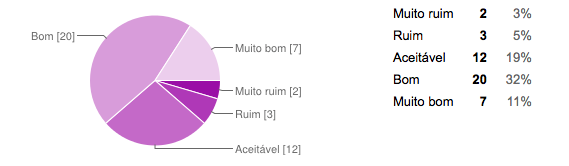
\includegraphics[width=14cm]{images/graficos/questao11.png}
  \caption{Gráfico de resultados da questão 11}
  \label{fig:questao11}
\end{center}
\end{figure}

\textbf{Comentários:}

Umas das grandes propostas do aplicativo foi fazer com que seus usuários pudessem acompanhar o deslocamento dos ônibus em, praticamente, tempo real. Com o intuito de avaliar se o aplicativo atende tal requisito, a questão 11 tem o propósito de mostrar se os usuários concordam com a localização dos ônibus mostrada no aplicativo, bem como com o intervalo de atualização da posição destes. 
	
Os dados mostrados na figura \figref{fig:questao11} revelam que, dos 44 usuários avaliados, 12 informaram que o tempo de atualização pode ser considerado aceitável, 20 acreditam que o tempo de atualização é bom e 7 consideram esse intervalo de tempo muito bom. Nesse sentido, conclui-se que a maioria dos participantes da pesquisa acharam que o intervalo de tempo de atualização é, no mínimo, aceitável.\newline

\textbf{Questão 12: A utilização do FindBus ajuda a estimar o exato momento que seu ônibus vai chegar no ponto?}

\begin{center}
\begin{longtable}{c|c|c}
\hline
    \multicolumn{1}{c}{\textbf{Resultado}} & \multicolumn{1}{c}{\textbf{Quantidade}} & \multicolumn{1}{c}{\textbf{Percentual}} \\
\hline
    Ajuda totalmente & 14 &  22\%\\
    \hline
    Ajuda parcialmente & 28 & 44\%\\
    \hline
    Não ajuda & 2 &  3\%\\
    \hline

\caption{Tabela de resultados obtidos na questão 12}
\label{tabq12}
\end{longtable}
\end{center}


\begin{figure}[h]
\begin{center}
  \includegraphics[width=15cm]{images/graficos/questao12.png}
  \caption{Gráfico de resultados da questão 12}
  \label{fig:questao12}
\end{center}
\end{figure}

\textbf{Comentários:}

Esta questão foi desenvolvida com a finalidade de atestar se o aplicativo fornece subsídios suficientes para que os usuários consigam estimar o exato momento que seu veículo chegará ao ponto de ônibus. 
Analisando os dados contidos na tabela X, observa-se que 22\% dos avaliados consideram que o aplicativo ajuda totalmente a prever o momento que o ônibus vai chegar no ponto, 44\% acreditam que o aplicativo ajuda, no entanto, de maneira parcial, enquanto que apenas 3\% informaram que o sistema não ajuda a fazer essa estimativa. Isto posto, pode-se afirmar que, para a maioria dos usuários, a utilização do aplicativo ajuda de alguma forma a estimar o momento que o ônibus vai chegar no ponto.\newline

\textbf{Questão 13: Você acredita que o aplicativo ajuda a diminuir o risco de roubo, furto, estupros, sequestro e atropelamento que cotidianamente acontecem nos pontos? Isto é, sabendo a localização do ônibus e tendo uma estimativa de quando este chegará ao ponto é possível diminuir a insegurança nos pontos de ônibus? }

\begin{center}
\begin{longtable}{c|c|c}
\hline
    \multicolumn{1}{c}{\textbf{Resultado}} & \multicolumn{1}{c}{\textbf{Quantidade}} & \multicolumn{1}{c}{\textbf{Percentual}} \\
\hline
    Ajuda totalmente & 18 &  29\%\\
    \hline
    Ajuda parcialmente & 23 & 37\%\\
    \hline
    Não ajuda & 3 &  5\%\\
    \hline

\caption{Tabela de resultados obtidos na questão 13}
\label{tabq13}
\end{longtable}
\end{center}


\begin{figure}[h]
\begin{center}
  \includegraphics[width=16cm]{images/graficos/questao13.png}
  \caption{Gráfico de resultados da questão 13}
  \label{fig:questao13}
\end{center}
\end{figure}

\textbf{Comentários:}

Uma das grandes motivações para o desenvolvimento deste trabalho foi diminuir o número de pessoas suscetíveis a assaltos, bem como a outros incidentes nos pontos de ônibus. No primeiro capitulo deste trabalho, constatou-se a insatisfação da população no tocante a insegurança existente nos pontos, bem como como que o principal causador dessa insegurança era a falta de informação, sobretudo, sobre o momento que o veículo vai chegar no ponto. 
Isto posto, a questão 13 foi criada com o intuito de validar se o aplicativo ajuda, através da informação disponibilizada e, por conseguinte, do apoio a tomada de decisões fornecido, a diminuir a insegurança, bem como os incidentes que costumeiramente ocorre nos pontos e terminais de ônibus.
O gráfico mostrado na figura \figref{fig:questao13} deixa claro que, para a maioria dos avaliados, a aplicação ajuda de alguma forma a diminuir as ocorrências de delitos nos pontos, onde 29\% afirmaram que a aplicação ajuda totalmente na luta contra insegurança, 37\% consideraram que o sistema ajuda parcialmente, enquanto 5\% acreditaram que a utilização da aplicação não ajuda a diminuir o números de incidentes nos terminais e pontos de ônibus.\newline


\textbf{Questão 14: A forma como é projetada a tarefa de inserir novos incidentes de trânsito lhe motiva a colaborar?}

\begin{center}
\begin{longtable}{c|c|c}
\hline
    \multicolumn{1}{c}{\textbf{Resultado}} & \multicolumn{1}{c}{\textbf{Quantidade}} & \multicolumn{1}{c}{\textbf{Percentual}} \\
\hline
    Sim & 38 &  60\%\\
    \hline
    Não & 6 & 10\%\\
    \hline
\caption{Tabela de resultados obtidos na questão 14}
\label{tabq14}
\end{longtable}
\end{center}


\begin{figure}[h]
\begin{center}
  \includegraphics[width=16cm]{images/graficos/questao14.png}
  \caption{Gráfico de resultados da questão 14}
  \label{fig:questao14}
\end{center}
\end{figure}

\textbf{Comentários:}

Um dos pontos chaves da aplicação é a colaboração do usuário com cadastros de ocorrências de incidentes de  trânsito, através destas é possível recomendar as melhores linhas, informar tudo que está acontecendo na cidade, bem como fazer com que os usuários tomem as melhores decisões sobre como, onde e qual ônibus utilizar. Contudo, para que tudo isso aconteça, faz-se necessário que o usuário se sinta motivado a cadastrar uma ocorrência, exatamente como fora discutido no capítulo \ref{ch:crowdsourcing} deste trabalho. Para tanto, esta questão teve como objetivo saber se a forma como a tarefa de cadastrar uma nova ocorrência motiva os usuários a colaborarem com os problemas que estão vivenciando no trânsito.     
	
Os dados revelam que 38 dos 44 avaliados consideraram que a forma como a tarefa de cadastrar novos incidentes foi projetada acaba motivando a colaboração do usuário. Nesse sentido, pode-se afirmar que a maioria dos usuários do aplicativo se sentem motivados a colaborar com a divulgação dos incidentes que estão vivenciando.\newline

\textbf{Questão 15: Depois de receber uma notificação de proximidade do seu ônibus, como você classifica o tempo que você tem para se deslocar para o ponto?}

\begin{center}
\begin{longtable}{c|c|c}
\hline
    \multicolumn{1}{c}{\textbf{Resultado}} & \multicolumn{1}{c}{\textbf{Quantidade}} & \multicolumn{1}{c}{\textbf{Percentual}} \\
\hline
    1 & 1 &  2\%\\
    \hline
    2 & 1 & 2\%\\
    \hline
    3 & 7 &  11\%\\
    \hline
    4 & 28 & 44\%\\
    \hline
    5 & 7 & 7\%\\
    \hline
\caption{Tabela de resultados obtidos na questão 15}
\label{tabq15}
\end{longtable}
\end{center}


\begin{figure}[h]
\begin{center}
  \includegraphics[width=16cm]{images/graficos/questao15.png}
  \caption{Gráfico de resultados da questão 15}
  \label{fig:questao15}
\end{center}
\end{figure}

\textbf{Comentários:}

Uma das funcionalidades do aplicativo é alertar o usuário quando um ônibus de uma linha que costumeiramente este utiliza está se aproximando. Todavia, além de notificar, é necessário que o alerta seja enviando com um tempo de antecedência que permita o usuário conseguir chegar ao ponto antes do ônibus passar. Para avaliar se esse ínterim é satisfatório, bem como se essa funcionalidade realmente funciona como fora especificada, a questão 15 permitiu que o participante da pesquisa classificasse o tempo para se deslocar para o ponto após uma notificação de proximidade com uma nota de 1 a 5, onde 1 significa uma classificação muito ruim e 5 uma avaliação muito boa.
	
Observa-se, no gráfico disponível na figura \figref{fig:questao15}, uma concentração maior na classificação 4, tendo poucas classificações consideras negativas. Assim, sendo possível afirmar que a maioria dos avaliados conseguem se deslocar até o ponto em um tempo hábil.\newline

\textbf{Questão 16: Com a ajuda do aplicativo você consegue saber quais linhas passam em um determinado ponto.}

\begin{center}
\begin{longtable}{c|c|c}
\hline
    \multicolumn{1}{c}{\textbf{Resultado}} & \multicolumn{1}{c}{\textbf{Quantidade}} & \multicolumn{1}{c}{\textbf{Percentual}} \\
\hline
    Concordo totalmente & 25 &  40\%\\
    \hline
    Concordo parcialmente & 17 & 27\%\\
    \hline
     Não concordo & 2 & 3\%\\
    \hline
\caption{Tabela de resultados obtidos na questão 16}
\label{tabq16}
\end{longtable}
\end{center}


\begin{figure}[h]
\begin{center}
  \includegraphics[width=16cm]{images/graficos/questao16.png}
  \caption{Gráfico de resultados da questão 16}
  \label{fig:questao16}
\end{center}
\end{figure}

\textbf{Comentários:}

Outra grande motivação deste trabalho foi melhorar o nível de informação disponível no tocante aos serviços do transporte público. No primeiro capítulo, foi mostrado que a maioria dos usuários de transporte público estão insatisfeitos com a qualidade das informações disponíveis nos terminais de ônibus, sendo uma das principais críticas a dificuldade de saber quais linhas passam por determinado ponto. 

Uma das propostas do aplicativo desenvolvido neste trabalho é informar aos usuários quais linhas passam por um determinado ponto escolhido por este. Todavia, faz-se necessário validar se realmente o sistema funciona como fora especificado. Para tanto, a questão 16 foi criada a fim de questionar aqueles que utilizam frequentemente a aplicação se eles concordam que a mesma consegue fornecer tal serviço.

Observa-se que 42 usuários, de um total de 44, afirmaram concordar com a afirmação feita na questão 16, o que significa dizer que 67\%, dos 70\% dos avaliados que avançaram para fase de avaliação, estão satisfeitos com informação disponibilizada pelo aplicativo no que tange a relação feita entre linhas e pontos de ônibus. \newline

\textbf{Questão 17: De modo geral, como você classifica a usabilidade do aplicativo?}

\begin{center}
\begin{longtable}{c|c|c}
\hline
    \multicolumn{1}{c}{\textbf{Resultado}} & \multicolumn{1}{c}{\textbf{Quantidade}} & \multicolumn{1}{c}{\textbf{Percentual}} \\
\hline
    1 & 3 &  5\%\\
    \hline
    2 & 0 & 0\%\\
    \hline
    3 & 5 &  8\%\\
    \hline
    4 & 30 & 48\%\\
    \hline
    5 & 6 & 10\%\\
    \hline
\caption{Tabela de resultados obtidos na questão 17}
\label{tabq17}
\end{longtable}
\end{center}


\begin{figure}[h]
\begin{center}
  \includegraphics[width=16cm]{images/graficos/questao17.png}
  \caption{Gráfico de resultados da questão 17}
  \label{fig:questao17}
\end{center}
\end{figure}

\textbf{Comentários:}

Umas das grandes preocupações e, sobretudo, um dos requisitos da proposta desenvolvida foi fazer com que a aplicação tivesse uma boa usabilidade, isto é, fosse simples e muito intuitiva, para que, desta forma, pudesse ser utilizada por todos usuários do transporte público. Para tanto, com o objetivo de medir se aplicação realmente atende a proposta, pediu-se aos avaliados que atribuísse uma nota de 1 a 5 para usabilidade do aplicativo, onde 1 significava que o sistema possui uma usabilidade muito ruim, enquanto que uma no 5 significava dizer que a aplicação tem uma usabilidade excelente.
	
Analisando o gráfico presente na figura \figref{fig:questao17}, nota-se a existência de algumas avaliações negativas. Não obstante, observa-se uma concentração bem maior na nota 4, o que acaba mostrando, também, que a maioria dos avaliados não estão totalmente satisfeitos e acreditam que a usabilidade ainda pode melhorar. \newline

\textbf{Questão 18: Você acredita que uma pessoa sem conhecimento técnico utilizaria o FindBus?}


\begin{center}
\begin{longtable}{c|c|c}
\hline
    \multicolumn{1}{c}{\textbf{Resultado}} & \multicolumn{1}{c}{\textbf{Quantidade}} & \multicolumn{1}{c}{\textbf{Percentual}} \\
\hline
    Sim & 41 &  65\%\\
    \hline
    Não & 3 & 5\%\\
    \hline
\caption{Tabela de resultados obtidos na questão 18}
\label{tabq18}
\end{longtable}
\end{center}

\begin{figure}[h]
\begin{center}
  \includegraphics[width=16cm]{images/graficos/questao18.png}
  \caption{Gráfico de resultados da questão 18}
  \label{fig:questao18}
\end{center}
\end{figure}

\textbf{Comentários:}

A questão 18 teve o objetivo de servir como um complemento da questão 17 de modo a contrapor as repostas das duas questões. Para tanto, parte-se da prerrogativa de que se uma pessoa sem nenhum conhecimento técnico consegue utilizar a aplicação, esta possui uma boa usabilidade. Nesse sentido, a questão 18 poderia tanto validar como invalidar o que fora respondido na questão 17.
	
Analisando os dados apresentados na tabela \ref{tabq17}, bem como os dados informados na tabela \ref{tabq18}, nota-se a mesma quantidade de respostas tanto para uma total insatisfação com a usabilidade do aplicativo quanto para não possibilidade de uma pessoa sem conhecimento técnico utilizar o sistema, o que mostra total coerência entre as repostas das duas questões.
	
Nota-se, no gráfico da figura \figref{fig:questao18}, que 65\% dos avaliados, dos 70\% que avançaram para fase de avaliação, afirmaram que mesmo uma pessoa sem conhecimento técnico conseguiria utilizar e usufruir de todos os recursos disponíveis na aplicação.\newline

\textbf{Questão 19: Avalie o FindBus com uma nota de 1 a 5.}


\begin{center}
\begin{longtable}{c|c|c}
\hline
    \multicolumn{1}{c}{\textbf{Resultado}} & \multicolumn{1}{c}{\textbf{Quantidade}} & \multicolumn{1}{c}{\textbf{Percentual}} \\
\hline
    1 & 2 &  3\%\\
    \hline
    2 & 1 & 2\%\\
    \hline
    3 & 3 &  5\%\\
    \hline
    4 & 19 & 30\%\\
    \hline
    5 & 19 & 30\%\\
    \hline
\caption{Tabela de resultados obtidos na questão 19}
\label{tabq19}
\end{longtable}
\end{center}

\begin{figure}[h]
\begin{center}
  \includegraphics[width=16cm]{images/graficos/questao19.png}
  \caption{Gráfico de resultados da questão 19}
  \label{fig:questao19}
\end{center}
\end{figure}

\textbf{Comentários:}

Por fim, com a finalidade de medir, de modo geral, a satisfação dos usuários com o aplicativo, pediu-se aos avaliados que dessem uma nota de 1 a 5, onde 1 significava uma total insatisfação e 5 uma total satisfação com o sistema. 
	
O gráfico mostrado na figura \figref{fig:questao19}, aponta uma grande concentração nas respostas 4 e 5, onde 19 avaliados atribuíram uma no 4 e 19 atribuíram uma nota 5, o que significa dizer que 38 usuários, dos 44 avaliados, estão satisfeitos com o uso do aplicativo.\newline

\section{Análise dos resultados}
\label{sc:analiseResultados}

A partir dos dados, bem como das analises parciais apresentadas na seção \ref{sc:apresentacaoResultados}. deste trabalho podemos concluir que, para o grupo avaliado, o aplicativo conseguiu cumprir com os objetivos gerais propostos na seção \ref{sc:objetivoGerais}, haja vista que a maioria dos usuários que participaram da pesquisa apresentaram respostas positivas em relação a utilização do aplicativo e, sobretudo, as informações fornecidas pelas principais funcionalidades deste.
	
Observa-se, através das respostas coletadas nas questões  2, 4, 6 e 7, que o aplicativo realmente consegue fazer com que os usuários visualizem, a priori, somente as informações no tocante ao transporte público e mobilidade de sua cidade, sendo, portanto, encaixado no contexto da cidade onde ele se encontra, conforme fora proposto no primeiro objetivo específico deste trabalho. 
	
Nota-se, também, analisando os dados apresentados na questão 14, que a forma como a tarefa de inserir novos incidentes de trânsito acaba estimulando a colaboração do usuário, visto que a maioria dos avaliados afirmaram sentirem-se motivados a colaborar com a divulgação dos problemas enfrentados durante o dia-a-dia da cidade. Isto posto, pode-se afirmar que segundo objetivo específico proposto neste trabalho também conseguiu ser atingido com o desenvolvimento da proposta.
	
Ademais, de acordo com os dados mostrados nas questões 4, 5, 10, 12 e 13, pode-se afirmar que o aplicativo consegue realmente fazer com que seus usuários saibam a real localização de um determinado ônibus juntamente com informações de distâncias e linhas, podendo, desta forma, prever o exato momento que o ônibus passará em um determinado ponto e, por conseguinte, otimizar seu temo e ficar menos vulnerável a insegurança existente no pontos e terminais, exatamente como proposto no terceiro objetivo específico deste trabalho. 

De modo a comprovar que o quarto objetivo específico deste trabalho foi atendido com o desenvolvimento da proposta, os dados da coletados na questão 11 foram analisados. Os dados mostram que a maioria dos avaliados consideraram o tempo de atualização e localização dos ônibus aceitável, sendo possível monitorar o deslocamento do veículo em, praticamente, tempo real.
	
O quinto objetivo específico deste trabalho propusera que a proposta permitisse que o usuário visualizasse todas as rotas, linhas e pontos de ônibus da cidade onde ele se encontra, bem como saber quais linhas passam por um determinado ponto. Analisando os dados obtidos nas questões 6 e 16, observa-se uma grande quantidade de respostas positivas e, desta forma, apoiando-se nas analises parciais apresentadas nessas duas questões, pode-se afirmar que o aplicativo realmente consegue cumprir o objetivo proposto.
	
Outrossim, os dados coletados na questão 7, bem como a analise parcial feita no comentário da referida questão, mostram que os usuários conseguem cadastrar ocorrências de trânsito por eles vivenciadas, bem como visualizar as ocorrências cadastradas por outros usuários, validando, assim, o sexto e sétimo objetivos específicos apresentados na seção \ref{sc:objetivoEspecificos} deste trabalho.  
	
O oitavo objetivo específico deste trabalho propusera que a proposta desenvolvida fosse capaz de recomendar a melhor rota para que o usuário chegue ao seu destino. Assim sendo, as respostas obtidas nas questões 8 e 9, de acordo com a analise parcial realizada nessas questões, que mostra a discrepância existente entre o número de respostas positivas em relação as negativas, pode-se afirmar que aplicativo consegue, apoiando-se nas informações disponibilizadas pelos próprios usuários através da colaboração, recomendar as melhores linhas para que o usuário consiga chegar a um determinado destino.

	





